\documentclass{beamer}
\usecolortheme{dove}
\setbeamertemplate{navigation symbols}{}
\newenvironment{alltt}{\ttfamily}{\par}
\usepackage{amsmath,amssymb,amsfonts,amsthm, multicol, subfigure, color}
\usepackage{bm}
\usepackage{graphicx}
\usepackage{tabularx}
\usepackage{booktabs}
\usepackage{hyperref}
\usepackage{pdfpages}
\usepackage{xcolor}
\definecolor{dodgerblue}{rgb}{.118, .575, 1}
\definecolor{seagreen4}{RGB}{46, 139, 87}
\def\independenT#1#2{\mathrel{\rlap{$#1#2$}\mkern2mu{#1#2}}}
\newcommand\independent{\protect\mathpalette{\protect\independenT}{\perp}}
\newcommand\indep{\protect\mathpalette{\protect\independenT}{\perp}}
\def\logit{\text{logit}}
\usepackage{stackrel}
\usepackage{tikz}
\usetikzlibrary{arrows,shapes.arrows,positioning,shapes,patterns,calc}
\newcommand\slideref[1]{\vskip .1cm \scriptsize \textcolor{gray}{{#1}}}
\definecolor{seagreen}{RGB}{46, 139, 87}
\newcommand\red[1]{\color{red}#1}
\newcommand\blue[1]{\color{blue}#1}
\newcommand\gray[1]{\color{gray}#1}
\newcommand\green[1]{\color{olive}#1}
\newcommand\seagreen[1]{\color{seagreen}#1}
\newcommand\purple[1]{\color{purple}#1}
\newcommand\orange[1]{\color{orange}#1}
\newcommand\black[1]{\color{black}#1}
\newcommand\white[1]{\color{white}#1}
\newcommand\teal[1]{\color{teal}#1}
\newcommand\magenta[1]{\color{magenta}#1}
\newcommand\Fuchsia[1]{\color{Fuchsia}#1}
\newcommand\BlueGreen[1]{\color{BlueGreen}#1}
\newcommand\bblue[1]{\textcolor{blue}{\textbf{#1}}}
\newcommand\bred[1]{\textcolor{red}{\textbf{#1}}}
\newcommand\bgray[1]{\textcolor{gray}{\textbf{#1}}}
\newcommand\bgreen[1]{\textcolor{seagreen}{\textbf{#1}}}
\colorlet{lightgray}{gray!40}
\pgfdeclarelayer{bg}    % declare background layer for tikz
\pgfsetlayers{bg,main} % order layers for tikz
\newcommand\bref[2]{\href{#1}{\color{blue}{#2}}}
\newcommand\mycite[1]{\begin{scriptsize}\textcolor{darkgray}{(#1)}\end{scriptsize}}
\newcommand\iid{\stackrel{\text{iid}}{\sim}}
\newcommand\E{\text{E}}
\newcommand\V{\text{V}}
\renewcommand\P{\text{P}}
\newcommand{\Cov}{\text{Cov}}
\newcommand{\Cor}{\text{Cor}}
\newcommand\doop{\text{do}}
\newcommand{\tcframe}{\frame{
\small{
\only<1|handout:0>{\tableofcontents}
\only<2|handout:1>{\tableofcontents[currentsection]}}
}}
% Credit for the following to https://tex.stackexchange.com/questions/44983/beamer-removing-headline-and-its-space-on-a-single-frame-for-plan-but-keepin
\makeatletter
    \newenvironment{withoutheadline}{
        \setbeamertemplate{headline}[default]
        \def\beamer@entrycode{\vspace*{-\headheight}}
    }{}
\makeatother
\setbeamercovered{invisible}
\usepackage[round]{natbib}
\bibliographystyle{humannat-mod}
\setbeamertemplate{enumerate items}[default]
\usepackage{mathtools}
% BELOW THREE LINES MAKES NAME IN FOOTER
\setbeamertemplate{footline}[text line]{%
\parbox{\linewidth}{\vspace*{-8pt}Lundberg, Johnson, and Stewart. What is Your Estimand?}}%\hfill\insertshortauthor\hfill\insertpagenumber}}

%\setbeamertemplate{footline}[text line]{%
%\parbox{\linewidth}{\vspace*{-8pt}Ian Lundberg (Princeton)}}%\hfill\insertshortauthor\hfill\insertpagenumber}}
%t\setbeamertemplate{navigation symbols}{}

% Make the header figure that will appear frequently
\newcommand\headerfigure{
\begin{tikzpicture}[x = \textwidth, y = \textheight, every node/.style={anchor = center}]
\node at (0,1) {\resizebox{\textwidth}{!}{\begin{tikzpicture}[x = 1.7in, y = .3in]
    \node[cloud, draw, align=center, cloud puffs=20,cloud puff arc=110, aspect=2, inner sep=.5mm, font = \small] (general) at (-.1,0) {Theory or\\general goal};
    %%%%%%%%%%
    \node[align=center, font = \small] (theoretical) at (1,0) {Theoretical\\estimand};
    \draw[->, thick] (general) -- (theoretical);
    \node[align = center, anchor = south, font = {\bf\small}] at (.5,0) {Set};
    \node[align = center, anchor = north, font = \small] at (.5,0) {by argument};
    %%%%%%%%%%
    \node[align=center, font = \small] (empirical) at (2,0) {Empirical\\estimand};
    \draw[->, thick] (theoretical) -- (empirical);
    \node[align = center, anchor = south, font = {\bf\small}] at (1.5,0) {Link};
    \node[align = center, anchor = north, font = \small] at (1.5,0) {by assumption};
    %%%%%%%%%%
    \node[align=center, font = \small] (estimate) at (3,0) {Estimation\\strategy};
    \draw[->, thick] (empirical) -- (estimate);
    \node[align = center, anchor = south, font = {\bf\small}] at (2.5,0) {Learn};
    \node[align = center, anchor = north, font = \small] at (2.5,0) {by data};
    \end{tikzpicture}
    }};
\end{tikzpicture}
}
% Make the versions that have only one step in black
\newcommand\headerfigureset{
\begin{tikzpicture}[x = \textwidth, y = \textheight, every node/.style={anchor = center}]
\node at (0,1) {\resizebox{\textwidth}{!}{\begin{tikzpicture}[x = 1.7in, y = .3in]
    \node[cloud, draw, align=center, cloud puffs=20,cloud puff arc=110, aspect=2, inner sep=.5mm, font = \small] (general) at (-.1,0) {Theory or\\general goal};
    %%%%%%%%%%
    \node[align=center, font = \small] (theoretical) at (1,0) {Theoretical\\estimand};
    \draw[->, thick] (general) -- (theoretical);
    \node[align = center, anchor = south, font = {\bf\small}] at (.5,0) {Set};
    \node[align = center, anchor = north, font = \small] at (.5,0) {by argument};
    %%%%%%%%%%
    \node[align=center, font = \small, gray] (empirical) at (2,0) {Empirical\\estimand};
    \draw[->, thick, gray] (theoretical) -- (empirical);
    \node[align = center, anchor = south, font = {\bf\small}, gray] at (1.5,0) {Link};
    \node[align = center, anchor = north, font = \small, gray] at (1.5,0) {by assumption};
    %%%%%%%%%%
    \node[align=center, font = \small, gray] (estimate) at (3,0) {Estimation\\strategy};
    \draw[->, thick, gray] (empirical) -- (estimate);
    \node[align = center, anchor = south, font = {\bf\small}, gray] at (2.5,0) {Learn};
    \node[align = center, anchor = north, font = \small, gray] at (2.5,0) {by data};
    \end{tikzpicture}
    }};
\end{tikzpicture}
}
\newcommand\headerfigurelink{
\begin{tikzpicture}[x = \textwidth, y = \textheight, every node/.style={anchor = center}]
\node at (0,1) {\resizebox{\textwidth}{!}{\begin{tikzpicture}[x = 1.7in, y = .3in]
    \node[cloud, draw, align=center, cloud puffs=20,cloud puff arc=110, aspect=2, inner sep=.5mm, font = \small, gray] (general) at (-.1,0) {Theory or\\general goal};
    %%%%%%%%%%
    \node[align=center, font = \small] (theoretical) at (1,0) {Theoretical\\estimand};
    \draw[->, thick, gray] (general) -- (theoretical);
    \node[align = center, anchor = south, font = {\bf\small}, gray] at (.5,0) {Set};
    \node[align = center, anchor = north, font = \small, gray] at (.5,0) {by argument};
    %%%%%%%%%%
    \node[align=center, font = \small] (empirical) at (2,0) {Empirical\\estimand};
    \draw[->, thick] (theoretical) -- (empirical);
    \node[align = center, anchor = south, font = {\bf\small}] at (1.5,0) {Link};
    \node[align = center, anchor = north, font = \small] at (1.5,0) {by assumption};
    %%%%%%%%%%
    \node[align=center, font = \small, gray] (estimate) at (3,0) {Estimation\\strategy};
    \draw[->, thick, gray] (empirical) -- (estimate);
    \node[align = center, anchor = south, font = {\bf\small}, gray] at (2.5,0) {Learn};
    \node[align = center, anchor = north, font = \small, gray] at (2.5,0) {by data};
    \end{tikzpicture}
    }};
\end{tikzpicture}
}
\newcommand\headerfigurelearn{
\begin{tikzpicture}[x = \textwidth, y = \textheight, every node/.style={anchor = center}]
\node at (0,1) {\resizebox{\textwidth}{!}{\begin{tikzpicture}[x = 1.7in, y = .3in]
    \node[cloud, draw, align=center, cloud puffs=20,cloud puff arc=110, aspect=2, inner sep=.5mm, font = \small, gray] (general) at (-.1,0) {Theory or\\general goal};
    %%%%%%%%%%
    \node[align=center, font = \small, gray] (theoretical) at (1,0) {Theoretical\\estimand};
    \draw[->, thick, gray] (general) -- (theoretical);
    \node[align = center, anchor = south, font = {\bf\small}, gray] at (.5,0) {Set};
    \node[align = center, anchor = north, font = \small, gray] at (.5,0) {by argument};
    %%%%%%%%%%
    \node[align=center, font = \small] (empirical) at (2,0) {Empirical\\estimand};
    \draw[->, thick, gray] (theoretical) -- (empirical);
    \node[align = center, anchor = south, font = {\bf\small}, gray] at (1.5,0) {Link};
    \node[align = center, anchor = north, font = \small, gray] at (1.5,0) {by assumption};
    %%%%%%%%%%
    \node[align=center, font = \small] (estimate) at (3,0) {Estimation\\strategy};
    \draw[->, thick] (empirical) -- (estimate);
    \node[align = center, anchor = south, font = {\bf\small}] at (2.5,0) {Learn};
    \node[align = center, anchor = north, font = \small] at (2.5,0) {by data};
    \end{tikzpicture}
    }};
\end{tikzpicture}
}

\newcommand\estimandFigure{

\begin{tikzpicture}[x = \textwidth, y = \textheight, every node/.style={anchor = center}]
%\node at (0,1) {\resizebox{\textwidth}{!}{\begin{tikzpicture}[x = 1.7in, y = .3in]
\node<10->[circle, fill = lightgray, draw = lightgray, font = \footnotesize, inner sep = 8pt] (point1) at (.18,.55) {};
\node<10->[gray, font = \footnotesize, align = center, anchor = north] (usqNote) at (point1.south) {A \bgray{unit-specific}\\\bgray{quantity}};
\node[circle, fill = lightgray, draw = lightgray, font = \footnotesize, inner sep = 8pt] (point2) at (.33,.5) {};
\node[circle, fill = lightgray, draw = lightgray, font = \footnotesize, inner sep = 8pt] (point3) at (.25,.35) {};
\node[circle, fill = lightgray, draw = lightgray, font = \footnotesize, inner sep = 8pt] (point4) at (.4,.38) {};
\node[circle, fill = lightgray, draw = lightgray, font = \footnotesize, inner sep = 8pt] (point5) at (.12,.37) {};
\node[circle, fill = lightgray, draw = lightgray, font = \footnotesize, inner sep = 8pt] (point6) at (.45,.55) {};
\draw[line width = 2pt, gray, rounded corners] (.05,.3) rectangle (.5,.6);
\node[gray, font = \footnotesize, align = left, anchor = south west] at (.5,.3) {Averaged over a\\\bgray{target population}};
\node[font = \scriptsize] at (point1) {$Y_i(t)$};
\node[font = \scriptsize] at (point2) {$Y_i(t)$};
\node[font = \scriptsize] at (point3) {$Y_i(t)$};
\node[font = \scriptsize] at (point4) {$Y_i(t)$};
\node[font = \scriptsize] at (point5) {$Y_i(t)$};
\node[font = \scriptsize] at (point6) {$Y_i(t)$};
    \end{tikzpicture}
    %}};
%\end{tikzpicture}
}

\newcommand\estimandFigureBottomCaption{

\begin{tikzpicture}[x = \textwidth, y = \textheight, every node/.style={anchor = center}]
%\node at (0,1) {\resizebox{\textwidth}{!}{\begin{tikzpicture}[x = 1.7in, y = .3in]
\node[circle, fill = lightgray, draw = lightgray, font = \footnotesize, inner sep = 8pt] (point1) at (.18,.55) {};
\node[gray, font = \footnotesize, align = center, anchor = north] (usqNote) at (point1.south) {A \bgray{unit-specific}\\\bgray{quantity}};
\node[circle, fill = lightgray, draw = lightgray, font = \footnotesize, inner sep = 8pt] (point2) at (.33,.5) {};
\node[circle, fill = lightgray, draw = lightgray, font = \footnotesize, inner sep = 8pt] (point3) at (.25,.35) {};
\node[circle, fill = lightgray, draw = lightgray, font = \footnotesize, inner sep = 8pt] (point4) at (.4,.38) {};
\node[circle, fill = lightgray, draw = lightgray, font = \footnotesize, inner sep = 8pt] (point5) at (.12,.37) {};
\node[circle, fill = lightgray, draw = lightgray, font = \footnotesize, inner sep = 8pt] (point6) at (.45,.55) {};
\draw[line width = 2pt, gray, rounded corners] (.05,.3) rectangle (.5,.6);
\node[gray, font = \footnotesize, align = center, anchor = north] at (.275,.3) {Averaged over a\\\bgray{target population}};
\node[font = \scriptsize] at (point1) {$Y_i(t)$};
\node[font = \scriptsize] at (point2) {$Y_i(t)$};
\node[font = \scriptsize] at (point3) {$Y_i(t)$};
\node[font = \scriptsize] at (point4) {$Y_i(t)$};
\node[font = \scriptsize] at (point5) {$Y_i(t)$};
\node[font = \scriptsize] at (point6) {$Y_i(t)$};
    \end{tikzpicture}
    %}};
%\end{tikzpicture}
}

\newcommand\estimandFigureBottomCaptionCustom[5]{
\begin{tikzpicture}[x = #4\textwidth, y = #5\textheight, every node/.style={anchor = center}]
\node[circle, fill = lightgray, draw = lightgray, font = \footnotesize, inner sep = #3] (point1) at (.18,.55) {};
\node[gray, font = \footnotesize, align = center, anchor = north] (usqNote) at (point1.south) {A \bgray{unit-specific}\\\bgray{quantity}};
\node[circle, fill = lightgray, draw = lightgray, font = \footnotesize, inner sep = #3] (point2) at (.41,.5) {};
\node[circle, fill = lightgray, draw = lightgray, font = \footnotesize, inner sep = #3] (point3) at (.25,.35) {};
\node[circle, fill = lightgray, draw = lightgray, font = \footnotesize, inner sep = #3] (point4) at (.4,.38) {};
\node[circle, fill = lightgray, draw = lightgray, font = \footnotesize, inner sep = #3] (point5) at (.12,.37) {};
\draw[line width = 2pt, gray, rounded corners] (.05,.3) rectangle (.5,.6);
\node[gray, font = \footnotesize, align = center, anchor = north] at (.275,.3) {Averaged over a\\\bgray{target population}};
\node[font = #2, align = left] at (point1) {#1};
\node[font = #2, align = left] at (point2) {#1};
\node[font = #2, align = left] at (point3) {#1};
\node[font = #2, align = left] at (point4) {#1};
\node[font = #2, align = left] at (point5) {#1};
    \end{tikzpicture}
}

\newcommand\estimandFigureBottomCaptionCustomDiamond[5]{
\begin{tikzpicture}[x = #4\textwidth, y = #5\textheight, every node/.style={anchor = center}]
\node[diamond, fill = lightgray, draw = lightgray, font = \footnotesize, inner sep = #3] (point1) at (.18,.55) {};
\node[gray, font = \footnotesize, align = center, anchor = north] (usqNote) at (point1.south) {A \bgray{unit-specific}\\\bgray{quantity}};
\node[diamond, fill = lightgray, draw = lightgray, font = \footnotesize, inner sep = #3] (point2) at (.41,.5) {};
\node[diamond, fill = lightgray, draw = lightgray, font = \footnotesize, inner sep = #3] (point3) at (.25,.35) {};
\node[diamond, fill = lightgray, draw = lightgray, font = \footnotesize, inner sep = #3] (point4) at (.4,.38) {};
\node[diamond, fill = lightgray, draw = lightgray, font = \footnotesize, inner sep = #3] (point5) at (.12,.37) {};
\draw[line width = 2pt, gray, rounded corners] (.05,.3) rectangle (.5,.6);
\node[gray, font = \footnotesize, align = center, anchor = north] at (.275,.3) {Averaged over a\\\bgray{target population}};
\node[font = #2, align = left] at (point1) {#1};
\node[font = #2, align = left] at (point2) {#1};
\node[font = #2, align = left] at (point3) {#1};
\node[font = #2, align = left] at (point4) {#1};
\node[font = #2, align = left] at (point5) {#1};
    \end{tikzpicture}
}

\newcommand\estimandFigureBottomCaptionCustomPager[6]{
\begin{tikzpicture}[x = #4\textwidth, y = #5\textheight, every node/.style={anchor = center}]
\node[circle, fill = lightgray, draw = lightgray, font = \footnotesize, inner sep = #3] (point1) at (.18,.53) {};
\node[gray, font = \footnotesize, align = center, anchor = north] (usqNote) at (point1.south) {A \bgray{unit-specific}\\\bgray{quantity}};
\node[circle, fill = lightgray, draw = lightgray, font = \footnotesize, inner sep = #3] (point2) at (.4,.5) {};
\node[circle, fill = lightgray, draw = lightgray, font = \footnotesize, inner sep = #3] (point3) at (.32,.38) {};
\draw[line width = 2pt, gray, rounded corners] (.05,.3) rectangle (.5,.6);
\node[gray, font = \footnotesize, align = center, anchor = north] at (.275,.3) {#6};
\node[font = #2, align = left] at (point1) {#1};
\node[font = #2, align = left] at (point2) {#1};
\node[font = #2, align = left] at (point3) {#1};
    \end{tikzpicture}
}

\newcommand\estimandFigureBottomCaptionCustomPagerWhite[6]{
\begin{tikzpicture}[x = #4\textwidth, y = #5\textheight, every node/.style={anchor = center}]
\node[ellipse, fill = lightgray, draw = lightgray, font = \footnotesize] (point1) at (.31,.56) {$Y_i(\text{No record})$};
\node[gray, font = \footnotesize, align = center, anchor = north] (usqNote) at (point1.south) {A \bgray{unit-specific}\\\bgray{quantity}};
\node[ellipse, fill = lightgray, draw = lightgray, font = \footnotesize] (point2) at (.24,.43) {$Y_i(\text{No record})$};
\node[ellipse, fill = lightgray, draw = lightgray, font = \footnotesize] (point3) at (.31,.35) {$Y_i(\text{No record})$};
\draw[line width = 2pt, gray, rounded corners] (.05,.3) rectangle (.5,.6);
\node[gray, font = \footnotesize, align = center, anchor = north] at (.275,.3) {#6};
    \end{tikzpicture}
}

\newcommand\estimandFigureBottomCaptionCustomPagerBlack[6]{
\begin{tikzpicture}[x = #4\textwidth, y = #5\textheight, every node/.style={anchor = center}]
\node[rounded corners, fill = lightgray, draw = lightgray, font = \footnotesize] (point1) at (.24,.56) {$Y_i(\text{No record})$};
\node[gray, font = \footnotesize, align = center, anchor = north] (usqNote) at (point1.south) {A \bgray{unit-specific}\\\bgray{quantity}};
\node[rounded corners, fill = lightgray, draw = lightgray, font = \footnotesize] (point2) at (.31,.43) {$Y_i(\text{No record})$};
\node[rounded corners, fill = lightgray, draw = lightgray, font = \footnotesize] (point3) at (.24,.35) {$Y_i(\text{No record})$};
\draw[line width = 2pt, gray, rounded corners] (.05,.3) rectangle (.5,.6);
\node[gray, font = \footnotesize, align = center, anchor = north] at (.275,.3) {#6};
\end{tikzpicture}
}

\newcommand\estimandFigureNoCaptionCustom[5]{
\begin{tikzpicture}[x = #4\textwidth, y = #5\textheight, every node/.style={anchor = center}]
\node[circle, fill = lightgray, draw = lightgray, font = \footnotesize, inner sep = #3] (point1) at (.18,.53) {};
%\node[gray, font = \footnotesize, align = center, anchor = north] (usqNote) at (point1.south) {A \bgray{unit-specific}\\\bgray{quantity}};
\node[circle, fill = lightgray, draw = lightgray, font = \footnotesize, inner sep = #3] (point2) at (.41,.5) {};
\node[circle, fill = lightgray, draw = lightgray, font = \footnotesize, inner sep = #3] (point3) at (.25,.4) {};
\node[circle, fill = lightgray, draw = lightgray, font = \footnotesize, inner sep = #3] (point4) at (.4,.38) {};
\node[circle, fill = lightgray, draw = lightgray, font = \footnotesize, inner sep = #3] (point5) at (.12,.37) {};
\draw[line width = 2pt, gray, rounded corners] (.05,.3) rectangle (.5,.6);
%\node[gray, font = \footnotesize, align = center, anchor = north] at (.275,.3) {Averaged over a\\\bgray{target population}};
\node[font = #2, align = left] at (point1) {#1};
\node[font = #2, align = left] at (point2) {#1};
\node[font = #2, align = left] at (point3) {#1};
\node[font = #2, align = left] at (point4) {#1};
\node[font = #2, align = left] at (point5) {#1};
    \end{tikzpicture}
}

\newcommand\estimandFigureNoCaptionMissingA[5]{
\begin{tikzpicture}[x = #4\textwidth, y = #5\textheight, every node/.style={anchor = center}]
\node[circle, fill = lightgray, draw = black, line width = 1.3pt, font = \footnotesize, inner sep = #3] (point1) at (.18,.53) {};
\node[circle, fill = lightgray, draw = black, line width = 1.3pt, font = \footnotesize, inner sep = #3] (point2) at (.41,.5) {};
\node[circle, fill = lightgray, draw = black, line width = 1.3pt, font = \footnotesize, inner sep = #3] (point3) at (.25,.4) {};
\node[circle, fill = lightgray, draw = lightgray, font = \footnotesize, inner sep = #3] (point4) at (.4,.38) {};
\node[circle, fill = lightgray, draw = lightgray, font = \footnotesize, inner sep = #3] (point5) at (.12,.37) {};
\draw[line width = 2pt, gray, rounded corners] (.05,.3) rectangle (.5,.6);
%\node[gray, font = \footnotesize, align = center, anchor = north] at (.275,.3) {Averaged over a\\\bgray{target population}};
\node[font = #2, align = left] at (point1) {#1};
\node[font = #2, align = left] at (point2) {#1};
\node[font = #2, align = left] at (point3) {#1};
\node[font = #2, align = left] at (point4) {#1};
\node[font = #2, align = left] at (point5) {#1};
    \end{tikzpicture}
}

\newcommand\estimandFigureNoCaptionMissingB[5]{
\begin{tikzpicture}[x = #4\textwidth, y = #5\textheight, every node/.style={anchor = center}]
\node[circle, fill = lightgray, draw = lightgray, font = \footnotesize, inner sep = #3] (point1) at (.18,.53) {};
\node[circle, fill = lightgray, draw = lightgray, font = \footnotesize, inner sep = #3] (point2) at (.41,.5) {};
\node[circle, fill = lightgray, draw = lightgray, font = \footnotesize, inner sep = #3] (point3) at (.25,.4) {};
\node[circle, fill = lightgray, draw = black, line width = 1.3pt, font = \footnotesize, inner sep = #3] (point4) at (.4,.38) {};
\node[circle, fill = lightgray, draw = black, line width = 1.3pt, font = \footnotesize, inner sep = #3] (point5) at (.12,.37) {};
\draw[line width = 2pt, gray, rounded corners] (.05,.3) rectangle (.5,.6);
\node[font = #2, align = left] at (point1) {#1};
\node[font = #2, align = left] at (point2) {#1};
\node[font = #2, align = left] at (point3) {#1};
\node[font = #2, align = left] at (point4) {#1};
\node[font = #2, align = left] at (point5) {#1};
    \end{tikzpicture}
}

\newcommand\estimandFigureNoCaptionImputedA[5]{
\begin{tikzpicture}[x = #4\textwidth, y = #5\textheight, every node/.style={anchor = center}]
\node[circle, fill = lightgray, draw = black, line width = 1.3pt, font = \footnotesize, inner sep = #3] (point1) at (.18,.53) {};
\node[circle, fill = lightgray, draw = black, line width = 1.3pt, font = \footnotesize, inner sep = #3] (point2) at (.41,.5) {};
\node[circle, fill = lightgray, draw = black, line width = 1.3pt, font = \footnotesize, inner sep = #3] (point3) at (.25,.4) {};
\node[circle, fill = lightgray, draw = lightgray, font = \footnotesize, inner sep = #3] (point4) at (.4,.38) {};
\node[circle, fill = lightgray, draw = lightgray, font = \footnotesize, inner sep = #3] (point5) at (.12,.37) {};
\draw[line width = 2pt, gray, rounded corners] (.05,.3) rectangle (.5,.6);
%\node[gray, font = \footnotesize, align = center, anchor = north] at (.275,.3) {Averaged over a\\\bgray{target population}};
\node[font = #2, align = left] at (point1) {$Y_i(1)$};
\node[font = #2, align = left] at (point2) {$Y_i(1)$};
\node[font = #2, align = left] at (point3) {$Y_i(1)$};
\node[font = #2, align = left] at (point4) {$\hat{Y}_i(1)$};
\node[font = #2, align = left] at (point5) {$\hat{Y}_i(1)$};
    \end{tikzpicture}
}

\newcommand\estimandFigureNoCaptionImputedB[5]{
\begin{tikzpicture}[x = #4\textwidth, y = #5\textheight, every node/.style={anchor = center}]
\node[circle, fill = lightgray, draw = lightgray, font = \footnotesize, inner sep = #3] (point1) at (.18,.53) {};
\node[circle, fill = lightgray, draw = lightgray, font = \footnotesize, inner sep = #3] (point2) at (.41,.5) {};
\node[circle, fill = lightgray, draw = lightgray, font = \footnotesize, inner sep = #3] (point3) at (.25,.4) {};
\node[circle, fill = lightgray, draw = black, line width = 1.3pt, font = \footnotesize, inner sep = #3] (point4) at (.4,.38) {};
\node[circle, fill = lightgray, draw = black, line width = 1.3pt, font = \footnotesize, inner sep = #3] (point5) at (.12,.37) {};
\draw[line width = 2pt, gray, rounded corners] (.05,.3) rectangle (.5,.6);
\node[font = #2, align = left] at (point1) {$\hat{Y}_i(0)$};
\node[font = #2, align = left] at (point2) {$\hat{Y}_i(0)$};
\node[font = #2, align = left] at (point3) {$\hat{Y}_i(0)$};
\node[font = #2, align = left] at (point4) {$Y_i(0)$};
\node[font = #2, align = left] at (point5) {$Y_i(0)$};
    \end{tikzpicture}
}

\newcommand\estimandFigureSideCaptionCustom[5]{
\begin{tikzpicture}[x = #4\textwidth, y = #5\textheight, every node/.style={anchor = center}]
\node[circle, fill = lightgray, draw = lightgray, font = \footnotesize, inner sep = #3] (point1) at (.18,.48) {};
\node[gray, font = \footnotesize, align = center, anchor = north] (usqNote) at (point1.south) {A \bgray{unit-specific}\\\bgray{quantity}};
\node[circle, fill = lightgray, draw = lightgray, font = \footnotesize, inner sep = #3] (point2) at (.41,.53) {};
%\node[circle, fill = lightgray, draw = lightgray, font = \footnotesize, inner sep = #3] (point3) at (.25,.35) {};
\node[circle, fill = lightgray, draw = lightgray, font = \footnotesize, inner sep = #3] (point4) at (.38,.38) {};
%\node[circle, fill = lightgray, draw = lightgray, font = \footnotesize, inner sep = #3] (point5) at (.12,.37) {};
\draw[line width = 2pt, gray, rounded corners] (.05,.3) rectangle (.5,.6);
\node[gray, font = \footnotesize, align = left, anchor = south west] at (.5,.3) {Averaged over a\\\bgray{target population}};
\node[font = #2, align = left] at (point1) {#1};
\node[font = #2, align = left] at (point2) {#1};
%\node[font = #2, align = left] at (point3) {#1};
\node[font = #2, align = left] at (point4) {#1};
%\node[font = #2, align = left] at (point5) {#1};
    \end{tikzpicture}
}

\newcommand\roadmap[2]{
\begin{frame}[t]
\headerfigure
\begin{tikzpicture}[x = \textwidth, y = .8\textheight]
\node at (0,0) {};
\node at (1,1) {};
\node[anchor = north west, font = \large] (title) at (0.04,1) {\bgray{What is Your Estimand?} };
\node[anchor = north west, font = \small] (subtitle) at (title.south west) {Defining the Target Quantity Connects Statistical Evidence to Theory};
\draw[gray, line width = 2pt, line cap = rounded] (subtitle.south west) -- (subtitle.south east);
\node[anchor = north west, font = \small] (overview) at (0.04,.82) {\bgray{Introduce} a framework for quantitative social science};
\node[anchor = north west, font = \small] at (0.04,.75) {\bgray{Illustrate} through four examples. We have to:};
\node[anchor = north west, align = left, font = \footnotesize] (plan1) at (.08,.69) {1) Distinguish causal treatments from population labels};
\node[anchor = north west, align = left, font = \footnotesize] (plan2) at (.08,.64) {2) Recognize when empirical evidence is narrow};
\node[anchor = north west, align = left, font = \footnotesize] (plan3) at (.08,.59) {3) Address ambiguity about descriptive and causal claims};
\node[anchor = north west, align = left, font = \footnotesize] (plan4) at (.08,.54) {4) Beware of causal selection in descriptive claims};
%that causal selection can produce misleading description};
%\node[anchor = north west, align = left, font = \footnotesize] (plan4) at (.08,.54) {4) Beware that description without causal assumptions can mislead};
%\node[anchor = north west, align = left, font = \footnotesize] (plan4) at (.08,.54) {4) Beware that neglected causal selection can make description mislead};
%Beware of empirical regularities that mislead due to causal selection};
%that causal sample selection can make descriptive claims mislead};
%\node[anchor = north west, align = left, font = \footnotesize] (plan1) at (.08,.69) {1) An experiment where the links are very clear};
%\node[anchor = north west, align = left, font = \footnotesize] (plan2) at (.08,.64) {2) An instrumental variables design with a weak link to theory};
%\node[anchor = north west, align = left, font = \footnotesize] (plan3) at (.08,.59) {3) A demographic technique with an ambiguous link to theory};
%\node[anchor = north west, align = left, font = \footnotesize] (plan4) at (.08,.54) {4) An observational study with deeply misleading conclusions};
\node[anchor = north west, font = \small] at (0.04,.47) {\bgray{Document} widespread vagueness in \emph{ASR}};
\node[anchor = north west, font = \small] at (0.04,.4) {\bgray{Replicate} studies to demonstrate the framework in action};
\node[anchor = north west, font = \small] at (0.04,.33) {\bgray{Extend} to answer new theoretical questions};
\node[anchor = north west, align = left, font = \small] (discuss) at (0.04,.26) {\bgray{Discuss}}; 
\node[anchor = north west, align = left, font = \small] at (discuss.north east) {Every quantitative study\\should define the estimand};
\node[anchor = south east] at (1,-.02) {\resizebox{.3\textwidth}{!}{\estimandFigureBottomCaption{}{\normalsize}}};
\draw[->, line width = 1.5pt, blue] (0,#1) -- (#2,#1);
\end{tikzpicture}
\end{frame}
}

\title{\blue{Estimands in the study of inequality}}
\author{Ian Lundberg}
\date{Stewart Lab\\Princeton University\\7 October 2019}
%\date{Notestein Seminar\\Office of Population Research\\Princeton University\\15 October 2019}

\begin{document}

%\frame{\titlepage}

\begin{frame}
\centering
\begin{tikzpicture}[x = .5\textwidth, y = .5\textwidth]
\node at (-1,-1) {};
\node at (1,1) {};
\node[font = \LARGE, align = left, anchor = north west, blue] at (-1, .9) {\textbf{What is Your Estimand?}};
\node[font = \LARGE, align = left, anchor = north west] at (-1,.7) {Defining the Target Quantity\\Connects Statistical Evidence\\to Theory};
\node[anchor = north east] at (1,1) {\includegraphics[width = 1.3in]{output/target}};
%\node[anchor = north east] at (1, .9) {4 August 2020};
%\node[anchor = north east, align = right] at (1, .8) {Annual Meeting of the\\American Sociological\\Association};
\node[align = center, anchor = south east, align = left] (ian) at (-.56, .05) {Ian Lundberg};
\node[align = center, anchor = south] (rebecca) at (-.13,.05) {Rebecca Johnson};
\node[align = center, anchor = south west] (brandon) at (.3, .05) {Brandon M. Stewart};
\node[align = center, anchor = north, font = \scriptsize] (ianAffil) at (ian.south) {UCLA\\Sociology\\\bref{https://www.ianlundberg.org/}{ianlundberg.org}};%\\ilundberg@princeton.edu};
\node[align = center, anchor = north, font = \scriptsize] (rebeccaAffil) at (rebecca.south) {Dartmouth Quantitative\\Social Science\\\bref{https://www.rebeccajohnson.io/}{rebeccajohnson.io}};%\\rebecca.ann.johnson\\@dartmouth.edu};
\node[align = center, anchor = north, font = \scriptsize] (brandonAffil) at (brandon.south) {Princeton\\Sociology\\\bref{http://scholar.princeton.edu/bstewart}{brandonstewart.org}};%\\bms4@princeton.edu};
\node[align = left, anchor = south west, font = \scriptsize, text width = \textwidth] at (-1, -.65) {23 September 2021. \\%\emph{American Sociological Review}. Draft on \bref{https://doi.org/10.31235/osf.io/ba67n}{SocArxiv}. 
Replication code on  \bref{https://doi.org/10.7910/DVN/ASGOVU}{Dataverse}. Research reported in this publication was supported by The Eunice Kennedy Shriver National Institute of Child Health \& Human Development of the National Institutes of Health under Award Number P2CHD047879.};
\end{tikzpicture}
\end{frame}

\section{Intro}

% INTRO WITH HEADER APPEARING
\begin{frame}[t]
\only<1-18>{\phantom{\headerfigure}}
\only<19->{\headerfigure}
%\only<18,26->{\headerfigure}
%\only<19>{\headerfigureset}
%\only<20-22>{\headerfigurelink}
%\only<23-25>{\headerfigurelearn}
\begin{tikzpicture}[x = \textwidth, y = \textheight]
\node at (0,0) {};
\node at (1,.9) {};
\node<1-18>[anchor = north west, align = left] at (0,.9) {There is a question every quantitative study must answer:};
\node<2-18>[anchor = north, align = left, font = \large] at (.5,.8) {\bblue{What is your estimand?}};
\draw<3-18>[->, line width = 2pt, blue] (.615,.73) to[out = 270, in = 180] (.7,.65);
\node<3-18>[anchor = north east, align = right, font = \small] at (1,.7) {The \bgray{purpose} of the\\statistical analysis};
%\node<14->[anchor = north east, align = right, font = \small] at (1,.6) {stated \bgray{outside}\\of the model};
\node<4-13>[anchor = north west] at (0,.7) {A common answer:};
\node<5-13>[anchor = north west] at (0,.63) {--- We took [data source]};
\node<6-13>[anchor = north west] at (0,.57) {--- We estimated $\beta_1$};
\node<6-13>[anchor = north west] at (0,.5) {$Y = \beta_0 + X_1\beta_1 + X_2\beta_2 + \epsilon$};
\draw<7-13>[->, thick, gray] (.22, .4) -- (.22, .44);
\node<7-13>[anchor = north, align = center, font = \footnotesize, gray] at (.22,.4) {$\beta_1$ is an estimand\\that assumes a model};
%\node<8-10>[anchor = north west, align = center] at (0,.26) {What if the model is wrong?};
\node<8-13>[anchor = north west, align = left, font = \footnotesize, fill = seagreen4, fill opacity = .2, text opacity = 1, rounded corners] at (.45,.58) {What if the\\model is wrong?};
\node<9-13>[anchor = north east, align = right, font = \footnotesize, fill = gray, rounded corners, fill opacity = .25, text opacity = 1] at (1,.52) {The model is an\\approximation};
\node<10-13>[anchor = north west, align = left, font = \footnotesize, fill = seagreen4, rounded corners, fill opacity = .2, text opacity = 1] at (.45,.46) {So $\beta_1$ is an\\approximation to...};
\node<11-13>[anchor = north east, align = right, font = \footnotesize, fill = gray, rounded corners, fill opacity = .2, text opacity = 1] at (1,.4) {Something. I just\\haven't said what.};
\node<12-13>[anchor = north west, align = left, font = \footnotesize, fill = seagreen4, rounded corners, fill opacity = .2, text opacity = 1] at (.45,.34) {Is it a good\\approximation?};
\node<13>[anchor = north east, align = right, font = \footnotesize, fill = gray, rounded corners, fill opacity = .2, text opacity = 1] at (1,.28) {\bred{Epistemological}\\\bred{crisis}};
%\node<9-10>[anchor = north west, align = center] at (0,.2) {\bred{Epistemological crisis.}};
% Begin the proposed estimand statement
\node<15->[circle, fill = lightgray, draw = lightgray, font = \footnotesize, inner sep = 8pt] (point1) at (.18,.6) {};
\node<16>[font = \scriptsize] at (point1) {$Y_i$};
\node<17>[font = \scriptsize] at (point1) {$Y_i(t)$};
\node<15->[gray, font = \footnotesize, align = center, anchor = north] (usqNote) at (point1.south) {A \bgray{unit-specific}\\\bgray{quantity}};
\node<18->[circle, fill = lightgray, draw = lightgray, font = \footnotesize, inner sep = 8pt] (point2) at (.33,.55) {};
\node<18->[circle, fill = lightgray, draw = lightgray, font = \footnotesize, inner sep = 8pt] (point3) at (.25,.4) {};
\node<18->[circle, fill = lightgray, draw = lightgray, font = \footnotesize, inner sep = 8pt] (point4) at (.4,.43) {};
\node<18->[circle, fill = lightgray, draw = lightgray, font = \footnotesize, inner sep = 8pt] (point5) at (.12,.42) {};
\node<18->[circle, fill = lightgray, draw = lightgray, font = \footnotesize, inner sep = 8pt] (point6) at (.45,.6) {};
\draw<18->[line width = 2pt, gray, rounded corners] (.05,.35) rectangle (.5,.65);
\node<18->[gray, font = \footnotesize, align = center, anchor = north] at (.275,.35) {Aggregated over a\\\bgray{target population}};
\node<18->[font = \scriptsize] at (point1) {$Y_1(t)$};
\node<18-23>[font = \scriptsize] at (point2) {$Y_2(t)$};
\node<18->[font = \scriptsize] at (point3) {$Y_5(t)$};
\node<18-23>[font = \scriptsize] at (point4) {$Y_6(t)$};
\node<18-23>[font = \scriptsize] at (point5) {$Y_4(t)$};
\node<18->[font = \scriptsize] at (point6) {$Y_3(t)$};
% 19. Set.
\node<20->[font = \Large] at (.275,.75) {\bgray{Set}};
% 20. Link
% Link to observables
\node<21->[circle, draw = black, font = \footnotesize, inner sep = 8pt, line width = 2pt] at (point1) {};
\node<21->[circle, draw = black, font = \footnotesize, inner sep = 8pt, line width = 2pt] at (point3) {};
\node<21->[circle, draw = black, font = \footnotesize, inner sep = 8pt, line width = 2pt] at (point6) {};
\node<22->[font = \Large] at (.62,.75) {\bgray{Link}};
\node<22-> (x) at (.55,.6) {$\vec{X}$};
\node<22-> (t) at (.62,.6) {$T$};
\node<22-> (y) at (.69,.6) {$Y$};
\draw<22->[->, thick] (x) -- (t);
\draw<22->[->, thick] (t) -- (y);
\draw<22->[->, thick] (x) to[bend left] (y);
% Learn from data
\node<23->[font = \Large] at (.9,.75) {\bgray{Learn}};
\node<23-> (learnEquation) at (.9,.6) {$\hat{Y}_i(t) = \hat{f}(\vec{X}_i,t)$};
\node<24->[font = \scriptsize] at (point2) {$\hat{Y}_2(t)$};
\node<24->[font = \scriptsize] at (point4) {$\hat{Y}_6(t)$};
\node<24->[font = \scriptsize] at (point5) {$\hat{Y}_4(t)$};
\end{tikzpicture}
\end{frame}
% Possibly bring back gray references

% ROADMAP HERE
% We have done (1), about to start (2)
\begin{frame}[t]
\headerfigure
\begin{tikzpicture}[x = \textwidth, y = .8\textheight]
\node at (0,1) {};
\node[anchor = west] at (0,.8) {Roadmap of the talk:};
\node[anchor = west] at (.05,.65) {1) Examples of how things can go wrong};
\node[anchor = west] at (.05,.55) {2) An example that follows our framework from top to bottom};
\node at (1,0) {};
\end{tikzpicture}
\end{frame}

\begin{frame}[t]
\headerfigure \vskip 1in
Example 1: An influential study with a narrow theoretical estimand
\end{frame}

% Angrist and Evans
\begin{frame}[t]
\headerfigure
\begin{tikzpicture}[x = \textwidth, y = .8\textheight]
\node at (0,1.03) {};
\node at (1,0) {};
\node[anchor = south east, gray] at (1,.02) {Angrist and Evans 1998};
\node<2-9>[anchor = north west, font = \small, align = left] at (0, .9) {Effect of motherhood\\on employment};
\node<3-9>[font = \footnotesize, align = center] (z) at (.25,.32) {First two births\\are the same sex};
\node<4-9>[font = \footnotesize] (t) at (.5,.32) {Third birth};
\draw<4-9>[->, thick] (z) -- (t);
\node<5-9>[font = \footnotesize] (y) at (.7,.32) {Employed};
\node<5-9>[font = \footnotesize, anchor = north] (u) at (.6,.45) {$U$};
\draw<5-9>[->, thick] (t) -- (y);
\draw<5-9>[->, thick] (u) -- (y);
\draw<5-9>[->, thick] (u) -- (t);
\node<6-9>[anchor = north west, gray, font = \bf] at (0,.97) {Vague estimand};
\node<7->[anchor = north west, gray, font = \bf] at (.37,.97) {Precise estimand};
\node<8->[anchor = north west, text width = .6\textwidth, font = \small, align = left] (precise1) at (.37,.9) {Effect of having \only<8>{\bblue{3 vs.~2 children}}\only<9->{3 vs.~2 children}};
\node<8>[anchor = north east, font = {\bf\footnotesize}, blue, align = center] (contrast) at (1,1.03) {unit-specific\\quantity};
\draw<8>[->, line width = 2pt, blue] (contrast) to[out = 180, in = 90] (.77,.89);
\node<9->[anchor = north west, text width = .6\textwidth, font = \small, align = left] at (.37, .84) {among those with at least two children who would have a third birth if and only if the first two were of the same sex};
\node<9>[anchor = south, font = {\bf\footnotesize}, seagreen] (population) at (.15,.6) {target population};
\draw<9>[->, line width = 2pt, seagreen] (population) to[out = 90, in = 180] (.35,.75);
\draw<9>[line width = 2pt, seagreen] (.38, .83) -- (.36, .83) -- (.36, .67) -- (.38,.67);
\draw<9>[line width = 2pt, seagreen] (.97, .83) -- (.99, .83) -- (.99, .67) -- (.97,.67);
\node<10->[font = \Large] at (.675,.6) {$\approx$ 4\% of all mothers};
%\node<10->[anchor = east] at (1,.3) {\resizebox{.35\textwidth}{!}{\estimandFigureBottomCaptionCustom{$Y_i(3)$\\$- Y_i(2)$}{\tiny}{8pt}{1}{1}}};
\node<11->[anchor = north west] at (0,.5) {\bgray{You have to argue either:}};
\node<11->[anchor = north west, font = \small] at (0,.4) {1)};
\node<12->[anchor = north west, font = \small] at (0.05,.4) {That estimand matters for theory, or};
%\node<13->[anchor = north west, font = \small] at (0.12,.4) {This 4\% of mothers is theoretically meaningful.};
\node<11->[anchor = north west, font = \small] at (0,.3) {2)};
\node<13->[anchor = north west, font = \small] at (0.05,.3) {It speaks to some broader estimand};
\end{tikzpicture}
\end{frame}

\begin{frame}[t]
\headerfigure \vskip 1in
Example 2: An influential study with a misleading link to evidence
\end{frame}

% FRYER
\begin{frame}[t]
\headerfigure
    \begin{tikzpicture}[x = \textwidth, y = .8\textheight]
    \node at (0,0) {};
    \node at (1,1) {};
    \node[anchor = north west] at (0,1) {\includegraphics[width = .5\textwidth]{output/fryer_p1}};
    \node<2->[anchor = north east, draw = white, fill = gray, text = black, rounded corners, fill opacity = .2, text opacity = 1, align = left, font = \small] (quote) at (1,1) {It is the most surprising\\result of my career.\\};
    \node<2->[anchor = south east, font = \footnotesize] at (quote.south east) {--- Roland Fryer};
    \node<3->[anchor = east, rotate = 6] at (1,.65) {\includegraphics[width = .5\textwidth]{output/fryer_nytimes}};
    \node<4->[anchor = east, rotate = -8] at (1,.3) {\includegraphics[width = .5\textwidth]{output/fryer_myth_wsj}};
    \node<5->[anchor = east, rotate = 3] at (1,.2) {\includegraphics[width = .5\textwidth]{output/fryer_guardian}};
    \end{tikzpicture}
    \end{frame}
   
   \begin{frame}
   \headerfigure
    
\begin{tikzpicture}[x = \textwidth, y = .8\textheight]
    \node at (0,0) {};
    \node at (1,1) {};
    % Fryer example
    %\node<3>[anchor = north west, align = left] at (0,.8) {\bgray{Example:} Police-involved shootings by race};
    \node[anchor = north west, font = {\bf\small}, gray, align = left] at (0,.97) {Evidence:};
    \node[anchor = north west, gray, font = {\bf\small}, align = left] (claimLabel) at (0,.82) {Claim:};
    \node[anchor = north west, gray, font = {\bf\small}, align = left] at (0,.72) {Why wrong:};
    \node[anchor = south east, gray, font = \footnotesize] at (1,0) {Fryer 2019. Fuller critique by Knox et al. 2020 and Durlauf and Heckman 2020.};
    \node<2->[anchor = north west, text width = 3in, font = {\small}] at  (.2, .97) {Police use lethal force at the same rate against black and white civilians who are stopped.};
    \node<3->[anchor = north west, text width = 3in, font = {\small}] (claimText) at  (.2,.82) {Police are unbiased};
    \node<10->[anchor = north west, text width = 3in, font = {\small}] (whyText) at (.2,.72) {Causal sample selection. Among those stopped, the white civilians may be more dangerous.};
    %\node<10->[anchor = north west, text width = 3in, font = {\small}] at (whyText.south west) {An unbiased officer might use \textbf{more} force against the white civlians.};
    \node<4-9>[anchor = center, align = center, font = \small] (d) at (.2,.35) {Perceived\\as black};
    \node<4-9>[anchor = center, align=center, font = \small] (y) at (.8,.35) {Lethal force};    
    \draw<4-9>[->, blue, line width = 2pt] (d) to[bend left = 22] (y);
    \node<5-9>[anchor = center, align=center, draw, rounded corners, font = \small] (c) at (.5,.35) {Stopped by\\police};
    \draw<5-9>[->, thick] (d) -- (c);
    \draw<5-9>[->, thick] (c) -- (y);
    \node<6-9>[anchor = center, font = \small] (u) at (.5,.15) {Criminal activity};
    \draw<6-9>[->, thick] (u) -- (c);
    \draw<6-9>[->, thick] (u) -- (y);
    % Visual depiction (will ultimately be its own clicks)
    \draw<7-9>[fill = white, draw = white] (0,.5) rectangle (1,1);
    % Perceived as white
    \node<7-9>[anchor = south, gray] at (.25,.85) {Perceived as \textbf{white}};
    \draw<7-9>[line width = 2pt, gray, line width = 2pt, rounded corners] (.1,.55) rectangle (.4,.85);
    \onslide<7>{
    \node[font = {\tiny\bf}, fill = red, rounded corners, line width = 2pt] at (.3,.8) {\textcolor{white}{Crime}};
    \node[font = {\tiny\bf}, fill = red, rounded corners, line width = 1pt] at (.3,.7) {\textcolor{white}{Crime}};
    \node[font = {\tiny\bf}, fill = gray, rounded corners, line width = 1pt] at (.3,.6) {\textcolor{white}{Safe}};
    \node[font = {\tiny\bf}, fill = gray, rounded corners, line width = 1pt] at (.2,.8) {\textcolor{white}{Safe}};
    \node[font = {\tiny\bf}, fill = gray, rounded corners, line width = 1pt] at (.2,.7) {\textcolor{white}{Safe}};
    \node[font = {\tiny\bf}, fill = gray, rounded corners, line width = 1pt] at (.2,.6) {\textcolor{white}{Safe}};
    }
    \onslide<8-9>{
    \node[font = {\tiny\bf}, draw = black, fill = red, rounded corners, line width = 1.5pt] at (.3,.8) {\textcolor{white}{Crime}};
    \node[font = {\tiny\bf}, draw = black, fill = red, rounded corners, line width = 1.5pt] at (.3,.7) {\textcolor{white}{Crime}};
    \node[opacity = .5, font = {\tiny\bf}, fill = gray, rounded corners, line width = 1.5pt] at (.3,.6) {\textcolor{white}{Safe}};
    \node[opacity = .5, font = {\tiny\bf}, fill = gray, rounded corners, line width = 1.5pt] at (.2,.8) {\textcolor{white}{Safe}};
    \node[opacity = .5, font = {\tiny\bf}, fill = gray, rounded corners, line width = 1.5pt] at (.2,.7) {\textcolor{white}{Safe}};
    \node[opacity = .5, font = {\tiny\bf}, fill = gray, rounded corners, line width = 1.5pt] at (.2,.6) {\textcolor{white}{Safe}};
    }
    % Perceived as black
    \node<7-9>[anchor = south, gray] at (.75,.85) {Perceived as \textbf{black}};
    \draw<7-9>[line width = 2pt, gray, line width = 2pt, rounded corners] (.6,.55) rectangle (.9,.85);
    \onslide<7-8>{
    \node[font = {\tiny\bf}, fill = red, rounded corners, line width = 1pt] at (.8,.8) {\textcolor{white}{Crime}};
    \node[font = {\tiny\bf}, fill = red, rounded corners, line width = 1pt] at (.8,.7) {\textcolor{white}{Crime}};
    \node[font = {\tiny\bf}, fill = gray, rounded corners, line width = 1pt] at (.7,.8) {\textcolor{white}{Safe}};
    \node[font = {\tiny\bf}, fill = gray, rounded corners, line width = 1pt] at (.7,.7) {\textcolor{white}{Safe}};
    \node[font = {\tiny\bf}, fill = gray, rounded corners, line width = 1pt] at (.8,.6) {\textcolor{white}{Safe}};
    \node[font = {\tiny\bf}, fill = gray, rounded corners, line width = 1pt] at (.7,.6) {\textcolor{white}{Safe}};
    }
    \onslide<9>{
    \node[draw = black, font = {\tiny\bf}, fill = red, rounded corners, line width = 1.5pt] at (.8,.8) {\textcolor{white}{Crime}};
    \node[draw = black, font = {\tiny\bf}, fill = red, rounded corners, line width = 1.5pt] at (.8,.7) {\textcolor{white}{Crime}};
    \node[draw = black, font = {\tiny\bf}, fill = gray, rounded corners, line width = 1.5pt] at (.7,.8) {\textcolor{white}{Safe}};
    \node[draw = black, font = {\tiny\bf}, fill = gray, rounded corners, line width = 1.5pt] at (.7,.7) {\textcolor{white}{Safe}};
    \node[opacity = .5, font = {\tiny\bf}, fill = gray, rounded corners, line width = 1.5pt] at (.8,.6) {\textcolor{white}{Safe}};
    \node[opacity = .5, font = {\tiny\bf}, fill = gray, rounded corners, line width = 1.5pt] at (.7,.6) {\textcolor{white}{Safe}};
    }
    % Fryer responds
    \node<11->[anchor = north west, gray, font = {\bf\small}, align = left] at (0,.47) {Fryer\\responds:};
    \draw<12->[thick] (claimLabel.west) -- (claimText.east);
    \node<13->[anchor = north west, draw = white, fill = gray, text = black, rounded corners, fill opacity = .2, text opacity = 1, align = left, font = \small, text width = 3in] at  (.2, .47) {``We use the term `racial differences' 114 times in lieu of the more prescriptive wording---`racial\\discrimination.' We use the phrase `conditional on an interaction' 20 times...I am not sure how many more ways we would have needed to caveat our results to satisfy [the critics].''};
    \end{tikzpicture}
\end{frame}

% BUCHMANN AND DIPRETE

\begin{frame}[t]
\headerfigure \vskip 1in
Example 3: An influential study where estimation led to confusion
\end{frame}

\begin{frame}[t]
\headerfigure \vskip .1in
%Example: Coefficients needlessly complicate descriptive estimands\vskip .1in
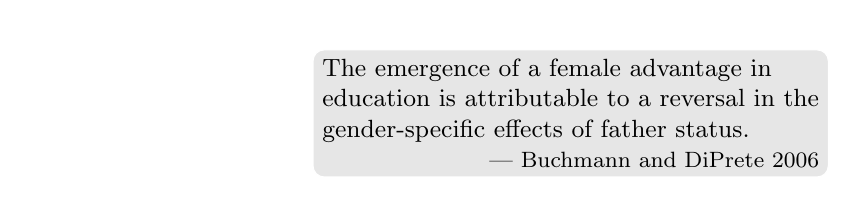
\begin{tikzpicture}
\node at (-3.5,.8) {};
\node<1->[anchor = north west, align = left, font = \small] at (0,1.91) {};
\node<1->[anchor = south west, draw = white, fill = gray, text = black, rounded corners, fill opacity = .2, text opacity = 1, align = left, font = \small] (quote) at (0,0) {The emergence of a female advantage in\\education is attributable to a reversal in the\\gender-specific effects of father status.\\};
\node<1->[anchor = south east, font = \footnotesize] at (quote.south east) {--- Buchmann and DiPrete 2006};
\end{tikzpicture}
\end{frame}

{
\setbeamertemplate{footline}[text line]{%
\parbox{\linewidth}{}}
\begin{frame}
\centering
\begin{tikzpicture}[x = \textwidth, y = \textheight]
%\includegraphics[height = \textheight]{output/buchmann_diprete_table}
\node[line width = 2pt, white] at (1.12,.39) {};
\node[line width = 2pt, white] at (.05,.39) {};
\node[anchor = north east] at (1,1) {\includegraphics[height = \textheight]{output/buchmann_diprete_table}};
\draw<2>[->, line width = 2pt, blue] (0.06,.394) -- (.11,.394);
\draw<2>[->, line width = 2pt, blue] (.7,.394) -- (.75,.394);
%\node[anchor = north west, align = left] (logit) at (-.1,1) {Logit\\predicting\\college\\completion};
%\node[anchor = north west, align = left, font = \footnotesize, gray] at (logit.south west) {Buchmann\\and\\DiPrete\\2006};
\end{tikzpicture}
\end{frame}
}
\begin{frame}[t]
\headerfigure \vskip .1in
%Example: Coefficients needlessly complicate descriptive estimands\vskip .1in
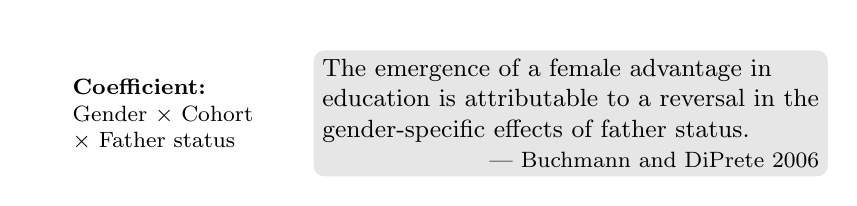
\begin{tikzpicture}
\node at (-3.5,.8) {};
\node<1->[anchor = north west, align = left, font = \small] at (0,1.91) {};
\node<1->[anchor = south west, draw = white, fill = gray, text = black, rounded corners, fill opacity = .2, text opacity = 1, align = left, font = \small] (quote) at (0,0) {The emergence of a female advantage in\\education is attributable to a reversal in the\\gender-specific effects of father status.\\};
\node<1->[anchor = south east, font = \footnotesize] at (quote.south east) {--- Buchmann and DiPrete 2006};
\node<1->[font = \footnotesize, align = left] (interaction) at (-1.9, .8) {\textbf{Coefficient:}\\Gender $\times$ Cohort\\$\times$ Father status};
%\node<2-3>[anchor = north west] at (-3.5, -.6) {\bgray{Outcome:}};
%\node<2-3>[anchor = north west] at (-1.3, -.6) {College completion};
%\node<2-3>[anchor = north west] at (-3.5, -1.1) {\bgray{Predictors:}};
%\node<2-3>[anchor = north west] at (-1.3, -1.1) {Gender, cohort, mother's education, father's education};
%\node<2>[anchor = north west, align = left] at (-3.5, -1.8) {\bgray{Descriptive}\\\bgray{estimand:}};
%\node<2>[anchor = north west, align = left] at (-1.3, -1.8) {Proportion completing college\\within subgroups of the predictors};
%\draw<2->[->, thick] (interaction) -- (-.2,.8);
\end{tikzpicture}
%Buchmann and DiPrete (2006): 
\resizebox{\textwidth}{!}{\begin{tikzpicture}[x = 6.5in, y = 1in]
\node<1>[anchor = north west] (A_plot) at (0,-.5) {\includegraphics{output/gss_fourPanel_set_stage}};
\node<2->[anchor = north west] (A_plot) at (0,-.5) {\includegraphics{output/gss_fourPanel_slideFigure}};
% Annotations on high completion group
%\draw[->, seagreen, thick] (.49,-1.45) to[bend left] (.47,-1.33);
%\draw[->, seagreen, thick] (.74,-1.4) to[bend right] (.75,-1.25);
% Annotations on groups with some disadvantage
\onslide<3->{
\draw[->, seagreen, thick] (.22,-2) to[bend left] (.13,-1.4);
\draw[->, seagreen, thick] (.22,-2.1) to[bend right] (.13,-2.35);
\draw[->, seagreen, thick] (.35,-2) -- (.45,-2);
\node[seagreen, fill = white, align = center, rounded corners, draw = seagreen] at (.285, -2.05) {Unusually high\\completion\\among men};
}
\end{tikzpicture}}
\onslide<4->{\bgray{Alternate theory}: The Vietnam War}
\end{frame}

\begin{frame}[t]
\headerfigure \vskip 1in
Meta-example: Vague estimands are widespread
\end{frame}

\begin{frame}[t]
\headerfigure
\resizebox{\textwidth}{!}{
    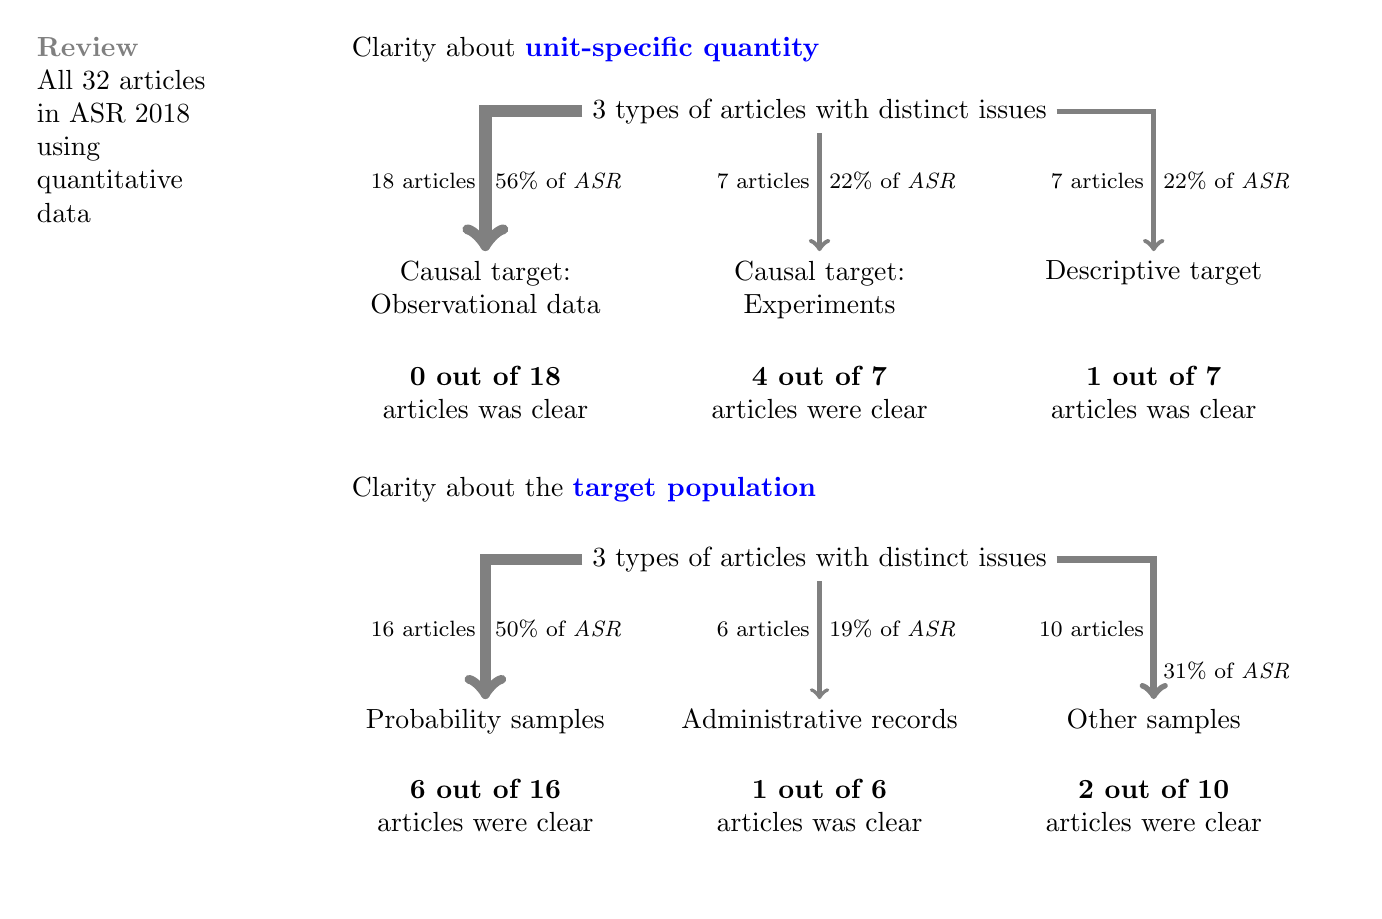
\begin{tikzpicture}[x = \textwidth, y = .7in]
    \node at (1.05,-6.5) {};
    %\draw[line width = 1.5pt] (asr.south west) -- (asr.south east);
    \node[align = left, anchor = north east, text width = 1in] (asr) at (-.1,-.4) {\bgray{Review}\\All 32 articles\\in ASR 2018\\using\\quantitative\\data};
    \node<2->[align = left, anchor = north west] at (0,-.4) {Clarity about \bblue{unit-specific quantity}};
    %\node[align = right, anchor = east] at (1,-.6) {Details in Appendix Table \ref{tab:causal_contrast_overview}};
    \node<2->[align = center] (three) at (.5,-1) {3 types of articles with distinct issues};
    \node<2->[align = center, anchor = north] (causal_observational) at (.15,-2) {Causal target:\\Observational data};
    \node<2->[align = center, anchor = north] (descriptive) at (.85,-2) {Descriptive target};
    \node<2->[align = center, anchor = north] (causal_experiments) at (.5,-2) {Causal target:\\Experiments};
    % Line widths are the percent multiplied by 8
    \draw<2->[->, line width = 4.48pt, gray] (three) -- (.15,-1) -- (causal_observational);
    \draw<2->[->, line width = 1.76pt, gray] (three) -- (causal_experiments);
    \draw<2->[->, line width = 1.76pt, gray] (three) -- (.85,-1) -- (descriptive);
    \node<2->[font = \footnotesize, anchor = east, align = right] at (.15,-1.5) {18 articles};
    \node<2->[font = \footnotesize, anchor = east, align = right] at (.5,-1.5) {7 articles};
    \node<2->[font = \footnotesize, anchor = east, align = right] at (.85,-1.5) {7 articles};
    \node<2->[font = \footnotesize, anchor = west, align = left] at (.15,-1.5) {56\% of \emph{ASR}};
    \node<2->[font = \footnotesize, anchor = west, align = left] at (.5,-1.5) {22\% of \emph{ASR}};
    \node<2->[font = \footnotesize, anchor = west, align = left] at (.85,-1.5) {22\% of \emph{ASR}};
    \node<3->[anchor = north, align = center] at (.15,-2.75) {\textbf{0 out of 18}\\articles was clear};
    \node<3->[anchor = north, align = center] at (.5,-2.75) {\textbf{4 out of 7}\\articles were clear};
    \node<3->[anchor = north, align = center] at (.85,-2.75) {\textbf{1 out of 7}\\articles was clear};
    %%%%%%%%%%%%%%%%%%%%%%%%%%%%%%%%%%
    \node<4->[anchor = west, align = left] at (0,-3.7) {Clarity about the \bblue{target population}};
    \node<4->[align = center] (three_target) at (.5,-4.2) {3 types of articles with distinct issues};
    \node<4->[align = center, anchor = north] (probability_samples) at (.15,-5.2) {Probability samples};
    \node<4->[align = center, anchor = north] (administrative_records) at (.5,-5.2) {Administrative records};
    \node<4->[align = center, anchor = north] (other_samples) at (.85,-5.2) {Other samples};
    \draw<4->[->, line width = 4pt, gray] (three_target) -- (.15,-4.2) -- (probability_samples);
    \draw<4->[->, line width = 1.5pt, gray] (three_target) -- (administrative_records);
    \draw<4->[->, line width = 2.48pt, gray] (three_target) -- (.85,-4.2) -- (other_samples);
    \node<4->[font = \footnotesize, anchor = east, align = right] at (.15,-4.7) {16 articles};
    \node<4->[font = \footnotesize, anchor = east, align = right] at (.5,-4.7) {6 articles};
    \node<4->[font = \footnotesize, anchor = east, align = right] at (.85,-4.7) {10 articles};
    \node<4->[font = \footnotesize, anchor = west, align = left] at (.15,-4.7) {50\% of \emph{ASR}};
    \node<4->[font = \footnotesize, anchor = west, align = left] at (.5,-4.7) {19\% of \emph{ASR}};
    \node<4->[font = \footnotesize, anchor = west, align = left] at (.85,-5) {31\% of \emph{ASR}};
    \node<5->[anchor = north, align = center] at (.15,-5.7) {\textbf{6 out of 16}\\articles were clear};
    \node<5->[anchor = north, align = center] at (.5,-5.7) {\textbf{1 out of 6}\\articles was clear};
    \node<5->[anchor = north, align = center] at (.85,-5.7) {\textbf{2 out of 10}\\articles were clear};
    %\node<12->[align = left, fill = white, draw = gray, line width = 2pt, rounded corners] at (.5,-3.5) {Lack of clarity\\--- Not clear what a study has shown\\--- How evidence informs theory is vague\\--- Not clear why results differ across studies};
    %\node<6->[align = left, anchor = north west, text width = 1.1in] (consequences) at (asr.south west) {\textcolor{white}{filler}\\\textcolor{white}{filler}\\\bgray{Confusion}\\arises about\\\only<7->{theory,}\only<8->{ methods,\\}\only<9->{ and conflicting\\studies.}};
    \end{tikzpicture}}
    \end{frame}
    
% TO DO MAKE THE PAPER REFERENCES VISIBLE HERE (THEY ARE TOO LOW)
\begin{frame}[t]
\headerfigure\vskip .5in
\begin{tikzpicture}[x = \textwidth, y = .8\textheight]
\node[anchor = west] at (0,.8) {Roadmap of the talk:};
\node[anchor = west] at (.05,.65) {1) Examples of how things can go wrong};
\node[anchor = west] at (.05,.55) {2) An example that follows our framework from top to bottom};
\end{tikzpicture} \pause

\begin{tikzpicture}[x = \textwidth, y = \textheight]
\node[anchor = west, align = left] (gce) at (0.2, .9) {The Gap-Closing Estimand:};
\node[anchor = west, align = left] (categories) at (0.2,.85) {The Disparity Across Social Categories};
\node[anchor = west, align = left] (treatment) at (0.2,.8) {That Would Persist if We Equalized a Treatment};
\node[anchor = east, align = right] at (.15, .88) {\bgray{General}};
\node[anchor = east, align = right] at (.15, .83) {\bgray{Method}};
\draw[line width = 2pt, gray, line cap = round] (.175,.78) -- (.175,.93);
\node[anchor = west, align = left] (gce) at (.2, .7) {Quantifying the Contribution of Occupational};
\node[anchor = west, align = left] (categories) at (.2,.65) {Segregation to Racial Disparities in Health:};
\node[anchor = west, align = left] (categories) at (.2,.6) {A Gap-Closing Perspective};
\node[anchor = east, align = right] at (.15, .68) {\bgray{Specific}};
\node[anchor = east, align = right] at (.15, .63) {\bgray{Example}};
\draw[line width = 2pt, gray, line cap = round] (.175,.73) -- (.175,.58);
\end{tikzpicture}
\end{frame}

% Gap-closing

% Maybe pull in ASA occupational segregation and health slides
% Scatterplot
% Theoretical estimand, with potential outcomes table
% Empirical estimand
% Estimation: the animated prediction thing
% SCATTERPLOT
\begin{frame}[t]
\headerfigure \vskip .1in
\label{descriptive_results}
\begin{tikzpicture}[x = \textwidth, y = \textheight]
\node at (0,0) {};
\node at (1,.8) {};
\node<1->[anchor = north east, font = \footnotesize, align = right, gray] (note1) at (1,.65) {Current\\Population Survey\\Annual Social and\\Economic Supplement\\Ages 25--60\\2005--2020};
%\node<2->[anchor = north east, font = \footnotesize] at (.33,.95) {Race};
%\node<2->[anchor = north east, font = \footnotesize] at (.33,.81) {Work-Limiting Disability};
%\node<3>[anchor = north west] at (0,.7) {\includegraphics[width = .68\textwidth]{figures/disability_by_race}};
%\node<4->[anchor = north east, font = \footnotesize] at (.33,.88) {Occupation};
%\node<5->[anchor = north west, font = \footnotesize] at (.35,.95) {(reported at year 1)};
%\node<5->[anchor = north west, font = \footnotesize] at (.35,.88) {(reported at year 1)};
%\node<6->[anchor = north west, font = \footnotesize] at (.35,.81) {(reported at year 2)};
\node<2>[anchor = north west] at (0,.7) {\includegraphics[width = .68\textwidth]{figures/scatter_factual_outcome_re_NonHispanicBlack_slide1}};
\node<3>[anchor = north west] at (0,.7) {\includegraphics[width = .68\textwidth]{figures/scatter_factual_outcome_re_NonHispanicBlack_slide2}};
\node<4>[anchor = north west] at (0,.7) {\includegraphics[width = .68\textwidth]{figures/scatter_factual_outcome_re_NonHispanicBlack_slide3}};
\node<5>[anchor = north west] at (0,.7) {\includegraphics[width = .68\textwidth]{figures/scatter_factual_outcome_re_NonHispanicBlack_slide4}};
\node<6>[anchor = north west] at (0,.7) {\includegraphics[width = .68\textwidth]{figures/scatter_factual_outcome_re_NonHispanicBlack_slide5}};
\node<7>[anchor = north west] at (0,.7) {\includegraphics[width = .68\textwidth]{figures/scatter_factual_outcome_re_NonHispanicBlack_slide6}};
\end{tikzpicture}
\end{frame}

% UPDATE THIS: Make this slide visual with the box and circles. Two theoretical estimands: factual and counterfactual
\begin{frame}[t]
\headerfigure \vskip .1in
Theoretical estimand \pause
\begin{itemize}
\item \bgray{Unit-specific quantity:}\\Onset of work-limiting disability\\if occupations were randomly shuffled\\within educational strata
\item Target population
\begin{itemize}
\item U.S. Ages 25--60
\item Employed at baseline survey
\item No work-limiting disability at baseline survey
\item Never previously quit a job for health reasons
\end{itemize}
\end{itemize}
\end{frame}

% DAG
\begin{frame}[t]
\headerfigure \vskip .1in
\centering
\begin{tikzpicture}[x = \textwidth, y = \textheight]
\node (l) at (.3,.5) {Covariates};
\node (x) at (.3,.7) {Race};
\node (t) at (.5,.6) {Occupation};
\node (y) at (.75,.6) {Health};
\draw[->, thick] (l) -- (t);
\draw[->, thick] (l) to[bend right = 15] (y);
\draw[->, line width = 2pt, blue] (t) -- (y);
\draw[->, thick] (x) -- (t);
\draw[->, thick] (x) -- (l);
\draw[->, thick] (x) to[bend left = 40] (y);
% Confounding of T is bad
\node<2>[red] (u) at (.5,.4) {$U$};
\draw<2>[->, red, line width = 2pt] (u) -- (t);
\draw<2>[->, red, line width = 2pt] (u) to[bend right = 20] (y); 
% Covariates
\node[anchor = north west, align = left, font = \footnotesize] (l_note) at (l.south west) {Sex, Age, Year\\Education\\Foreign born\\Self-rated health last year\\Employed\\No disability last year};
\end{tikzpicture}
\end{frame}

% After DAG, return to the table
\begin{frame}[t]
\headerfigure \vskip .1in

\begin{tikzpicture}[x = \textwidth, y = \textheight]
\node at (0,0) {};
%\node at (1,.75) {};
%\node[anchor = north] (how) at (.5, .95) {\bgray{A Counterfactual Setting:} Eliminate occupational segregation};
%\draw[line width = 2pt, gray, line cap = round] (how.south west) -- (how.south east);
\node[anchor = south, font = \footnotesize, rotate = 90] at (.05, .375) {\bgray{White}};
\node[anchor = south, font = \footnotesize, rotate = 90] at (0.05, .175) {\bgray{Black}};
\node[anchor = east, font = \footnotesize] at (.2, .45) {Person 1};
\node[anchor = east, font = \footnotesize] at (.2, .4) {Person 2};
\node[anchor = east, font = \footnotesize] at (.2, .35) {Person 3};
\node[anchor = east, font = \footnotesize] at (.2, .3) {Person 4};
\draw[thick, dashed] (.05,.275) -- (.75,.275);
\node[anchor = east, font = \footnotesize] at (.2, .25) {Person 5};
\node[anchor = east, font = \footnotesize] at (.2, .2) {Person 6};
\node[anchor = east, font = \footnotesize] at (.2, .15) {Person 7};
\node[anchor = east, font = \footnotesize] at (.2, .1) {Person 8};
\node[anchor = south, font = \footnotesize, align = center] at (.3, .5) {Administrative\\Assistant};
\node[anchor = south, font = \footnotesize, align = center] at (.5, .5) {Home Health\\Aid};
\node[anchor = south, font = \footnotesize, align = center] at (.7, .5) {Sales\\Supervisor};
\node (1a) at (.3, .45) {};
\node (2a) at (.3, .4) {};
\node (3a) at (.3, .35) {};
\node (4a) at (.3, .3) {};
\node (5a) at (.3, .25) {};
\node (6a) at (.3, .2) {};
\node (7a) at (.3, .15) {};
\node (8a) at (.3, .1) {};
\node (1b) at (.5, .45) {};
\node (2b) at (.5, .4) {};
\node (3b) at (.5, .35) {};
\node (4b) at (.5, .3) {};
\node (5b) at (.5, .25) {};
\node (6b) at (.5, .2) {};
\node (7b) at (.5, .15) {};
\node (8b) at (.5, .1) {};
\node (1c) at (.7, .45) {};
\node (2c) at (.7, .4) {};
\node (3c) at (.7, .35) {};
\node (4c) at (.7, .3) {};
\node (5c) at (.7, .25) {};
\node (6c) at (.7, .2) {};
\node (7c) at (.7, .15) {};
\node (8c) at (.7, .1) {};
\node<1-4>[font = \footnotesize] at (1a) {$y$};
\node<4-> at (.5,.65) {$\hat{y}_i(t) = \hat{f}(\vec{X}_i,t)$};
\onslide<1-5>{
\node[font = \footnotesize] at (6a) {$y$};
\node[font = \footnotesize] at (7a) {$y$};
\node[font = \footnotesize] at (3b) {$y$};
\node[font = \footnotesize] at (4b) {$y$};
\node[font = \footnotesize] at (2c) {$y$};
\node[font = \footnotesize] at (5c) {$y$};
\node[font = \footnotesize] at (8c) {$y$};
}
\onslide<2-4>{
\node[font = \tiny] at (1b) {$\bullet$};
\node[font = \tiny] at (1c) {$\bullet$};
}
\node<1-2>[font = \small, align = center, white] at (.9, .65) {Average outcome\\if occupations\\were shuffled};
\node<3->[font = \small, align = center] at (.9, .65) {Average outcome\\if occupations\\were shuffled};
\draw<3->[->, thick] (.9,.55) --  (.9,.5);
\draw<3-5>[rounded corners, fill = gray, fill opacity = .2] (.25,.425) rectangle (.75, .475);
\node<3-4>[font = \tiny] at (.9, .45) {$\bullet$};
\node<5->[font = \footnotesize] at (.9, .45) {$\hat{\bar{y}}$};
\onslide<5->{
\node[font = \footnotesize] at (1a) {$\hat{y}$};
\node[font = \footnotesize] at (1b) {$\hat{y}$};
\node[font = \footnotesize] at (1c) {$\hat{y}$};
}
\onslide<2-5>{
\node[font = \tiny] at (2a) {$\bullet$};
\node[font = \tiny] at (3a) {$\bullet$};
\node[font = \tiny] at (4a) {$\bullet$};
\node[font = \tiny] at (5a) {$\bullet$};
\node[font = \tiny] at (8a) {$\bullet$};
\node[font = \tiny] at (2b) {$\bullet$};
\node[font = \tiny] at (5b) {$\bullet$};
\node[font = \tiny] at (6b) {$\bullet$};
\node[font = \tiny] at (7b) {$\bullet$};
\node[font = \tiny] at (8b) {$\bullet$};
\node[font = \tiny] at (3c) {$\bullet$};
\node[font = \tiny] at (4c) {$\bullet$};
\node[font = \tiny] at (6c) {$\bullet$};
\node[font = \tiny] at (7c) {$\bullet$};
}
\onslide<6->{
\node[font = \footnotesize] at (2a) {$\hat{y}$};
\node[font = \footnotesize] at (3a) {$\hat{y}$};
\node[font = \footnotesize] at (4a) {$\hat{y}$};
\node[font = \footnotesize] at (5a) {$\hat{y}$};
\node[font = \footnotesize] at (6a) {$\hat{y}$};
\node[font = \footnotesize] at (7a) {$\hat{y}$};
\node[font = \footnotesize] at (8a) {$\hat{y}$};
\node[font = \footnotesize] at (2b) {$\hat{y}$};
\node[font = \footnotesize] at (3b) {$\hat{y}$};
\node[font = \footnotesize] at (4b) {$\hat{y}$};
\node[font = \footnotesize] at (5b) {$\hat{y}$};
\node[font = \footnotesize] at (6b) {$\hat{y}$};
\node[font = \footnotesize] at (7b) {$\hat{y}$};
\node[font = \footnotesize] at (8b) {$\hat{y}$};
\node[font = \footnotesize] at (2c) {$\hat{y}$};
\node[font = \footnotesize] at (3c) {$\hat{y}$};
\node[font = \footnotesize] at (4c) {$\hat{y}$};
\node[font = \footnotesize] at (5c) {$\hat{y}$};
\node[font = \footnotesize] at (6c) {$\hat{y}$};
\node[font = \footnotesize] at (7c) {$\hat{y}$};
\node[font = \footnotesize] at (8c) {$\hat{y}$};
}
\only<6->{
\node[font = \footnotesize] at (.9, .4) {$\hat{\bar{y}}$};
\node[font = \footnotesize] at (.9, .35) {$\hat{\bar{y}}$};
\node[font = \footnotesize] at (.9, .3) {$\hat{\bar{y}}$};
\node[font = \footnotesize] at (.9, .25) {$\hat{\bar{y}}$};
\node[font = \footnotesize] at (.9, .2) {$\hat{\bar{y}}$};
\node[font = \footnotesize] at (.9, .15) {$\hat{\bar{y}}$};
\node[font = \footnotesize] at (.9, .1) {$\hat{\bar{y}}$};
}
\draw<7->[rounded corners, fill = gray, fill opacity = .2] (.87,.28) rectangle (.93, .47);
\draw<7->[rounded corners, fill = gray, fill opacity = .2] (.87,.08) rectangle (.93, .27);
\node<7->[font = {\small\bf}, gray, align = center] at (.9,0) {Gap-Closing\\Estimand};
\end{tikzpicture}
\end{frame}

\begin{frame}[t]
\headerfigure \vskip .1in
\includegraphics<1>[width = \textwidth]{figures/segregation_slide_0}
\includegraphics<2>[width = \textwidth]{figures/segregation_slide_1}
\includegraphics<3>[width = \textwidth]{figures/segregation_slide_2}
\includegraphics<4>[width = \textwidth]{figures/segregation_slide_3}
\end{frame}

\begin{frame}[t]
\headerfigure
\begin{tikzpicture}[x = \textwidth, y = \textheight]
\node at (0,0)  {};
\node at (1,.8) {};
% Begin science table
\node<1>[anchor = north west] at (.05,.77) {
\scalebox{.7}{\begin{tikzpicture}[x = .9in, y = .3in, every node/.style={anchor = center}]
\node at (-1,-4) {};
\node at (0,2) {};
\node[anchor = south, align = center, font = \bf, gray, rotate = 90] at (-.5,-3.5) {Population};
\node at (0,-1) {Person 1};
\node at (0,-2) {Person 2};
\node at (0,-3) {Person 3};
\node at (0,-4) {Person 4};
\node at (0,-5) {Person 5};
\node at (0,-6) {Person 6};
\node[font = \bf, gray] at (1.5,1) {Treatment Condition};
\node at (1,0) {Black};
\node at (2,0) {White};
\draw[thick] (.6,-.5) -- (1.4,-.5);
\draw[thick] (1.6,-.5) -- (2.4,-.5);
\node at (1,-1) {$Y_1(\text{Black})$};
\node at (2,-1) {$Y_1(\text{White})$};
\node at (1,-2) {$Y_2(\text{Black})$};
\node at (2,-2) {$Y_2(\text{White})$};
\node at (1,-3) {$Y_3(\text{Black})$};
\node at (2,-3) {$Y_3(\text{White})$};
\node at (1,-4) {$Y_4(\text{Black})$};
\node at (2,-4) {$Y_4(\text{White})$};
\node at (1,-5) {$Y_5(\text{Black})$};
\node at (2,-5) {$Y_5(\text{White})$};
\node at (1,-6) {$Y_6(\text{Black})$};
\node at (2,-6) {$Y_6(\text{White})$};
\end{tikzpicture}}
};
\node<2->[anchor = north west] at (.05,.77) {
\scalebox{.7}{\begin{tikzpicture}[x = .9in, y = .3in, every node/.style={anchor = center}]
\node at (-1,-4) {};
\node at (0,2) {};
\node<2->[anchor = south, align = center, font = \bf, gray, rotate = 90] at (-.5,-2) {Black};
\node<2->[anchor = south, align = center, font = \bf, gray, rotate = 90] at (-.5,-5.5) {White};
\draw[line width = 1.2pt, gray] (-.45,-.7) -- (-.45,-3.3);
\draw[line width = 1.2pt, gray] (-.45,-4.2) -- (-.45,-6.8);
\node at (0,-1) {Person 1};
\node at (0,-2) {Person 2};
\node at (0,-3) {Person 3};
\node at (0,-4.5) {Person 4};
\node at (0,-5.5) {Person 5};
\node at (0,-6.5) {Person 6};
\only<3->{
\node[align = center] at (1,.4) {As\\observed};
\draw[thick] (.6,-.3) -- (1.4,-.3);
\node at (1,-1) {$Y_1$};
\node at (1,-2) {$Y_2$};
\node at (1,-3) {$Y_3$};
\node at (1,-4.5) {$Y_4$};
\node at (1,-5.5) {$Y_5$};
\node at (1,-6.5) {$Y_6$};
}
\only<4->{
\draw[draw = white, fill = gray, fill opacity = .2, rounded corners] (.7,-3.5) rectangle (1.3, -.5);
\draw[draw = white, fill = gray, fill opacity = .2, rounded corners] (.7,-7) rectangle (1.3, -4);
\node[anchor = north, font = \bf, gray, align = center] at (1,-7.3) {Descriptive\\Disparity};
}
\only<5->{
\draw[draw = white, fill = blue, fill opacity = .2, rounded corners] (1.7,-3.5) rectangle (2.3, -.5);
\draw[draw = white, fill = blue, fill opacity = .2, rounded corners] (1.7,-7) rectangle (2.3, -4);
\node<5->[anchor = north, font = \bf, blue, align = center, opacity = .5] at (2,-7.3) {Gap-Closing\\Estimand};
}
\only<5->{
\node[align = center] at (2,.4) {Under\\intervention};
\draw[thick] (1.6,-.3) -- (2.4,-.3);
\node at (2,-1) {$Y_1(t)$};
\node at (2,-2) {$Y_2(t)$};
\node at (2,-3) {$Y_3(t)$};
\node at (2,-4.5) {$Y_4(t)$};
\node at (2,-5.5) {$Y_5(t)$};
\node at (2,-6.5) {$Y_6(t)$};
}
\end{tikzpicture}}
};
%\node<6->[anchor = east, font = \footnotesize, align = center, draw = blue, draw opacity = .5, rounded corners, line width = 1pt] at (1,.7) {How much would\\the gap close\\if we intervene?};
\node<6->[anchor = south east, font = \scriptsize, align = left, gray] (c3) at (1,.15) {Lundberg 2021};
\only<6->{
\node[anchor = south east, font = \scriptsize, align = left, gray] (c2) at (c3.north east) {Jackson \& Vanderweele 2018};
\node[anchor = south east, font = \scriptsize, align = left, gray] (c1) at (c2.north east) {Vanderweele \& Robinson 2014};
}
\end{tikzpicture}
\end{frame}

% TO DO CLOSING. ARGUMENT ABOUT MATTERS FOR INEQUALITY

\begin{frame}[t]
\headerfigure

\begin{tikzpicture}[x = \textwidth, y = .8\textheight]
\node at (0,0) {};
\node at (1,1) {};
\node[anchor = north west, font = \Large] (question) at (0,1) {\bblue{What is your estimand?}};
\node<12->[anchor = north west, font = \small, align = left] at (question.south west) {Defining the Target Quantity\\Connects Statistical Evidence \\to Theory};
\node[anchor = north east, align = right, font = \small] (every) at (1,1) {Every quantitative study\\should answer this question};
\draw[->, line width = 1.7pt, blue] (.64,.965) -- (.59,.965);
\node[anchor = north east] at (1,.8) {\resizebox{1.5in}{!}{\estimandFigureBottomCaption}};
%\onslide<2>{
\node<2-3>[anchor = north west, align = left] at (0,.8) {When you \bblue{write} a quantitative paper,\\the estimand allows you to};
\node<3>[anchor = north west, font = \small] at (0,.65) {--- Motivate the question};
\node<3>[anchor = north west, font = \small] at (0,.58) {--- Address selection};
\node<3>[anchor = north west, font = \small] at (0,.51) {--- Use machine learning};
\node<3>[anchor = north west, font = \small] at (0,.44) {--- Speak to a broad audience};
%}
%\onslide<>{
\node<4-5>[anchor = north west, align = left] at (0,.8) {When you \bblue{read} a quantitative paper,\\the estimand allows you to};
\node<5>[anchor = north west, font = \small] at (0,.65) {--- Understand the author's aim};
\node<5>[anchor = north west, font = \small] at (0,.58) {--- Pinpoint your concerns};
%\node<8>[anchor = north west, align = left] at (0,.8) {When you \bblue{build on} a quantitative paper,\\the estimand allows you to};
%\node<8>[anchor = north west, font = \small] at (0,.65) {--- Relate one study to another};
%\node<8>[anchor = north west, font = \small] at (0,.58) {--- Build cumulatively on past work};
%}
%\node<13>[anchor = north west, align = left, font = \large] (key) at (0,.8) {The key:};
%\node<13>[anchor = north west, align = left, font = \large] at (key.north east) {Say precisely what you want\\to get from the data};
%\onslide<5>{
\node<6-9>[anchor = north west, align = left] at (0,.85) {\bblue{In the future,} estimands will\\only become more important};
\node<7-9>[anchor = north west, align = left] at (0,.7) {\bgray{New data} have missing values};
\node<7-9>[anchor = north west, font = \small] at (0,.63) {--- Non-probability samples};
\node<7-9>[anchor = north west, font = \small] at (0,.56) {--- Administrative records};
\node<8-9>[anchor = north west, align = left] at (0,.47) {\bgray{New methods} flourish with a clear goal};
\node<8-9>[anchor = north west, font = \small] at (0,.4) {--- Machine learning};
\node<9>[anchor = north west, align = left] at (0,.31) {\bgray{New questions} can be found beyond coefficients};
\node<9>[anchor = north west, font = \small] at (0,.24) {--- Describe counterfactual disparities};
\node<9>[anchor = north west, font = \small] at (0,.17) {--- Predict the effects of targeted interventions};
%\node<11>[anchor = north west, font = \small] at (0,.11) {--- Forecast future outcomes};
%}
%\onslide<6>{
%\node<12->[anchor = east] at (1,.5) {\estimandFigureBottomCaption};
\node<10->[anchor = west] (ian) at (0,.66) {\bgray{Ian Lundberg}};
\node<10->[anchor = north west, font = \footnotesize, align = left] at (ian.south west) {ilundberg@princeton.edu\\\blue{ianlundberg.org}};
\node<10->[anchor = west] (rebecca) at (0,.455) {\bgray{Rebecca Johnson}};
\node<10->[anchor = north west, font = \footnotesize, align = left] at (rebecca.south west) {rebecca.ann.johnson@\\dartmouth.edu\\\blue{rebeccajohnson.io}};
\node<10->[anchor = west] (brandon) at (0,.2) {\bgray{Brandon Stewart}};
\node<10->[anchor = north west, font = \footnotesize, align = left] at (brandon.south west) {bms4@princeton.edu\\\blue{brandonstewart.org}};
\node<10->[anchor = south east, align = right, font = \footnotesize, gray] (paper) at (1,0.034) {\emph{American Sociological Review}, 2021.\\Open access on \bref{https://doi.org/10.31235/osf.io/ba67n}{SocArxiv}\\Code on \bref{https://doi.org/10.7910/DVN/ASGOVU}{Dataverse}};
%\node<12->[anchor = north east, align = right, font = \small, gray] (paper) at (1,.4) {Forthcoming, \emph{American}\\\emph{Sociological Review}};
%\node<12>[anchor = north east, align = right, font = \small, gray] (draft) at (paper.south east) {Draft on \bref{https://doi.org/10.31235/osf.io/ba67n}{SocArxiv}};
%\node<12>[anchor = north east, align = right, font = \small, gray] (code) at (draft.south east) {Code on \bref{https://doi.org/10.7910/DVN/ASGOVU}{Dataverse}};
%}
\end{tikzpicture}
\end{frame}

\end{document}

% INTRO WITHOUT HEADER APPEARING
\begin{frame}
\begin{tikzpicture}[x = \textwidth, y = \textheight]
\node at (0,0) {};
\node at (1,1) {};
\node<1-18>[anchor = north west, align = left] at (0,.9) {There is a question every quantitative study must answer:};
\node<2-18>[anchor = north, align = left, font = \large] at (.5,.8) {\bblue{What is your estimand?}};
\draw<3-18>[->, line width = 2pt, blue] (.615,.73) to[out = 270, in = 180] (.7,.65);
\node<3-18>[anchor = north east, align = right, font = \small] at (1,.7) {The \bgray{purpose} of the\\statistical analysis};
%\node<14->[anchor = north east, align = right, font = \small] at (1,.6) {stated \bgray{outside}\\of the model};
\node<4-13>[anchor = north west] at (0,.7) {A common answer:};
\node<5-13>[anchor = north west] at (0,.63) {--- We took [data source]};
\node<6-13>[anchor = north west] at (0,.57) {--- We estimated $\beta_1$};
\node<6-13>[anchor = north west] at (0,.5) {$Y = \beta_0 + X_1\beta_1 + X_2\beta_2 + \epsilon$};
\draw<7-13>[->, thick, gray] (.22, .4) -- (.22, .44);
\node<7-13>[anchor = north, align = center, font = \footnotesize, gray] at (.22,.4) {$\beta_1$ is an estimand\\that assumes a model};
%\node<8-10>[anchor = north west, align = center] at (0,.26) {What if the model is wrong?};
\node<8-13>[anchor = north west, align = left, font = \footnotesize, fill = seagreen4, fill opacity = .2, text opacity = 1, rounded corners] at (.45,.55) {What if the\\model is wrong?};
\node<9-13>[anchor = north east, align = right, font = \footnotesize, fill = gray, rounded corners, fill opacity = .25, text opacity = 1] at (1,.47) {The model is an\\approximation};
\node<10-13>[anchor = north west, align = left, font = \footnotesize, fill = seagreen4, rounded corners, fill opacity = .2, text opacity = 1] at (.45,.39) {So $\beta_1$ is an\\approximation to...};
\node<11-13>[anchor = north east, align = right, font = \footnotesize, fill = gray, rounded corners, fill opacity = .2, text opacity = 1] at (1,.31) {Something. I just\\haven't said what.};
\node<12-13>[anchor = north west, align = left, font = \footnotesize, fill = seagreen4, rounded corners, fill opacity = .2, text opacity = 1] at (.45,.23) {Is it a good\\approximation?};
\node<13>[anchor = north east, align = right, font = \footnotesize, fill = gray, rounded corners, fill opacity = .2, text opacity = 1] at (1,.15) {\bred{Epistemological}\\\bred{crisis}};
%\node<9-10>[anchor = north west, align = center] at (0,.2) {\bred{Epistemological crisis.}};
% Begin the proposed estimand statement
\node<15->[circle, fill = lightgray, draw = lightgray, font = \footnotesize, inner sep = 8pt] (point1) at (.18,.6) {};
\node<16>[font = \scriptsize] at (point1) {$Y_i$};
\node<17>[font = \scriptsize] at (point1) {$Y_i(t)$};
\node<15->[gray, font = \footnotesize, align = center, anchor = north] (usqNote) at (point1.south) {A \bgray{unit-specific}\\\bgray{quantity}};
\node<18->[circle, fill = lightgray, draw = lightgray, font = \footnotesize, inner sep = 8pt] (point2) at (.33,.55) {};
\node<18->[circle, fill = lightgray, draw = lightgray, font = \footnotesize, inner sep = 8pt] (point3) at (.25,.4) {};
\node<18->[circle, fill = lightgray, draw = lightgray, font = \footnotesize, inner sep = 8pt] (point4) at (.4,.43) {};
\node<18->[circle, fill = lightgray, draw = lightgray, font = \footnotesize, inner sep = 8pt] (point5) at (.12,.42) {};
\node<18->[circle, fill = lightgray, draw = lightgray, font = \footnotesize, inner sep = 8pt] (point6) at (.45,.6) {};
\draw<18->[line width = 2pt, gray, rounded corners] (.05,.35) rectangle (.5,.65);
\node<18->[gray, font = \footnotesize, align = left, anchor = south west] at (.5,.35) {Aggregated over a\\\bgray{target population}};
\node<18->[font = \scriptsize] at (point1) {$Y_1(t)$};
\node<18-26>[font = \scriptsize] at (point2) {$Y_2(t)$};
\node<18->[font = \scriptsize] at (point3) {$Y_5(t)$};
\node<18-26>[font = \scriptsize] at (point4) {$Y_6(t)$};
\node<18-26>[font = \scriptsize] at (point5) {$Y_4(t)$};
\node<18->[font = \scriptsize] at (point6) {$Y_3(t)$};
% BEGIN FRAMEWORK
\node<20->[align=center, font = \small] (theoretical) at (.2,.9) {Theoretical\\estimand};
\node<20->[align=center, font = \small] (empirical) at (.5,.9) {Empirical\\estimand};
\node<20->[align=center, font = \small] (estimate) at (.8,.9) {Estimation\\strategy};
\draw<20->[->, thick] (theoretical) -- (empirical);
\draw<20->[->, thick] (empirical) -- (estimate);
\node<21->[align=center, font = \footnotesize] (set) at (.2,.75) {\textbf{Set}\\the target};
\draw<21->[->, thick] (set) -- (theoretical);
\node<22->[align=center, font = \footnotesize] (link) at (.5,.75) {\textbf{Link}\\to observables};
\draw<22->[->, thick] (link) -- (empirical);
\node<23->[circle, draw = black, font = \footnotesize, inner sep = 8pt, line width = 2pt] at (point1) {};
\node<23->[circle, draw = black, font = \footnotesize, inner sep = 8pt, line width = 2pt] at (point3) {};
\node<23->[circle, draw = black, font = \footnotesize, inner sep = 8pt, line width = 2pt] at (point6) {};
\node<24-> (x) at (.1,.2) {$X$};
\node<24-> (t) at (.25,.2) {$T$};
\node<24-> (y) at (.4,.2) {$Y$};
\draw<24->[->, thick] (x) -- (t);
\draw<24->[->, thick] (t) -- (y);
\draw<24->[->, thick] (x) to[bend left] (y);
\node<25->[align=center, font = \footnotesize] (learn) at (.8,.75) {\textbf{Learn}\\from data};
\draw<25->[->, thick] (learn) -- (estimate);
\node<26-> at (.75,.2) {$\hat{Y}_i(t) = \hat{f}(X_i,t)$};
\node<27>[font = \scriptsize] at (point2) {$\hat{Y}_2(t)$};
\node<27>[font = \scriptsize] at (point4) {$\hat{Y}_6(t)$};
\node<27>[font = \scriptsize] at (point5) {$\hat{Y}_4(t)$};
\end{tikzpicture}
\end{frame}
% POSSIBLE TO-DO: Make visualizations line up with set, link, learn in space
% Possibly bring back the gray references

\begin{frame}[t]
\headerfigure
\begin{tikzpicture}[x = \textwidth, y = \textheight]
\node at (0,.7) {};
\node at (0,0) {};
\node[font = \small, align = center] at (.25,.8) {Theory\\people};
\node[font = \small, align = center] at (.53,.8) {Causal\\people};
\node[font = \small, align = center] at (.8,.8) {Computational\\people};
\draw[thick] (.25, .85) -- (.25, .9);
\draw[thick] (.53, .85) -- (.53, .9);
\draw[thick] (.8, .85) -- (.8, .9);
\node[anchor = west] at (0,.7) {So...what is your estimand?};
% ESTIMAND VISUALIZATION
\node[gray, font = \footnotesize, align = center, anchor = north] (usqNote) at (point1.south) {A \bgray{unit-specific}\\\bgray{quantity}};
\node[circle, fill = lightgray, draw = lightgray, font = \footnotesize, inner sep = 8pt] (point2) at (.33,.55) {};
\node[circle, fill = lightgray, draw = lightgray, font = \footnotesize, inner sep = 8pt] (point3) at (.25,.4) {};
\node[circle, fill = lightgray, draw = lightgray, font = \footnotesize, inner sep = 8pt] (point4) at (.4,.43) {};
\node[circle, fill = lightgray, draw = lightgray, font = \footnotesize, inner sep = 8pt] (point5) at (.12,.42) {};
\node[circle, fill = lightgray, draw = lightgray, font = \footnotesize, inner sep = 8pt] (point6) at (.45,.6) {};
\draw[line width = 2pt, gray, rounded corners] (.05,.35) rectangle (.5,.65);
\node[gray, font = \footnotesize, align = left, anchor = south west] at (.5,.35) {Averaged over a\\\bgray{target population}};
\node[font = \scriptsize] at (point1) {$Y_i(t)$};
\node[font = \scriptsize] at (point2) {$Y_i(t)$};
\node[font = \scriptsize] at (point3) {$Y_i(t)$};
\node[font = \scriptsize] at (point4) {$Y_i(t)$};
\node[font = \scriptsize] at (point5) {$Y_i(t)$};
\node[font = \scriptsize] at (point6) {$Y_i(t)$};
    \end{tikzpicture}
% WHY CARE
\node[anchor = west] at (0,.3) {An explicit answer sets the path toward};
\node[anchor = west, font = \small] at (0,.2) {1) Transparent evidence and assumptions};
\node[anchor = west, font = \small] at (0,.15) {2) Use of machine learning};
\node[anchor = west, font = \small] at (0,.1) {3) Comprehension by a wide audience};
\end{tikzpicture}
\end{frame}

\begin{frame}[t]
\headerfigure
%Every quantitative paper should answer the question: what is your estimand? \vskip .2in
Benefits of our framework:
\begin{enumerate}
\item Transparent evidence and assumptions
\item Use of machine learning
\item Claims the public will understand
\end{enumerate}
\end{frame}


\end{document}